\documentclass{article}
 
\usepackage[preprint]{neurips_2020}
%preprint
%\usepackage{cite}

\usepackage{amsmath,amssymb,amsfonts}
\usepackage{algorithmic}
\usepackage{graphicx}
\usepackage{caption}
\usepackage{subcaption}
\usepackage{textcomp}
\usepackage{xcolor}
\usepackage{amsthm}
\usepackage{enumerate}
\usepackage{natbib}
\setcitestyle{numbers,square}
\usepackage{dsfont}
%\usepackage{siunitx}
%multi-row
\usepackage{multirow}
\usepackage{bbm}
\usepackage{bm}
\makeatletter
\newcommand{\Spvek}[2][r]{%
  \gdef\@VORNE{1}
  \left(\hskip-\arraycolsep%
    \begin{array}{#1}\vekSp@lten{#2}\end{array}%
  \hskip-\arraycolsep\right)}

\def\vekSp@lten#1{\xvekSp@lten#1;vekL@stLine;}
\def\vekL@stLine{vekL@stLine}
\def\xvekSp@lten#1;{\def\temp{#1}%
  \ifx\temp\vekL@stLine
  \else
    \ifnum\@VORNE=1\gdef\@VORNE{0}
    \else\@arraycr\fi%
    #1%
    \expandafter\xvekSp@lten
  \fi}
\makeatother

\def\pd{\partial}
\def\sen{\mathop{\rm sen}\nolimits} % seno
\def\senh{\mathop{\rm senh}\nolimits}
\def\N{\mathbb{N}}
\def\Z{\mathbb{Z}}
\def\Q{\mathbb{Q}}
\def\R{\mathbb{R}}
\def\C{\mathbb{C}} 

\newtheorem{Theorem}{Theorem}
\newtheorem{Proposition}{Proposition}
\newtheorem {Lemma}[Proposition] {Lemma}
\newtheorem {Corollary}[Proposition]{Corollary}
\newtheorem {Remark}[Proposition]{Remark}
\newtheorem {Example}{Example}[section]
\newtheorem {Definition}{Definition}[section]
\newtheorem {Figure}{Figure}[section]
\newcommand{\W}{\mathcal{W}}
\newcommand{\Deellip}{
\textit{DEEL.LIP}\footnote{https://github.com/deel-ai/deel-lip to be published soon}
}

\def\BibTeX{{\rm B\kern-.05em{\sc i\kern-.025em b}\kern-.08em
    T\kern-.1667em\lower.7ex\hbox{E}\kern-.125emX}}
\begin{document}

%\title{hinge regularized optimal transportation for robust classification}
\title{Achieving robustness in classification using optimal transport with hinge regularization}
\author{
  Mathieu Serrurier \\
  IRIT\\
  Universit\'{e} Paul Sabatier Toulouse
  \And
  Franck Mamalet\\
  IRT Saint-Exupery
 \And
  Alberto Gonz\'{a}lez-Sanz\\
  IMT\\
  Universit\'{e} Paul Sabatier Toulouse
  \And
  Thibaut Boissin\\
  IRT Saint-Exupery
 \And
  Jean-Michel Loubes \\
  IMT\\
  Universit\'{e} Paul Sabatier Toulouse
 \And
  Eustasio del Barrio \\
  Dpto. de Estad\'{\i}stica e Investigaci\'{o}n Operativa\\
  Universidad de Valladolid  
}
\maketitle
\begin{abstract}
We propose a new framework for robust binary classification, with Deep Neural Networks,  based on a hinge regularization of the Kantorovich-Rubinstein dual formulation for the estimation of the Wasserstein distance. The robustness of the approach is guaranteed by the strict Lipschitz constraint on functions required by the optimization problem and direct interpretation of the loss in terms of adversarial robustness. We prove that this classification formulation has a solution, and is still the dual formulation of an optimal transportation problem.  We also establish the geometrical properties of this optimal solution. We summarize  state-of-the-art methods to enforce Lipschitz constraints on neural networks and we propose new ones for convolutional networks (associated with an open source library for this purpose). The experiments show that the approach provides the expected guarantees in terms of robustness without any significant accuracy drop. The results also suggest that adversarial attacks on the proposed models visibly and meaningfully change the input, and can thus serve as an explanation for the classification.
% We also experimented adversarial attack on the proposed model, which suggests that visible and meaningfull changes must be made to the input in order to be mis-classified. This opens perspectives to 
%The results also suggest that adversarial attacks on the proposed models require to perform explicit change on the input critical part, and can thus serve as an explanation for the classification.
\end{abstract}
\section{Introduction}
\label{sec:intro}

The important progress in deep learning has led to a massive interest for these approaches in industry. However, when machine learning is applied for critical tasks such has in the transportation or the medical domain, empirical and theoretical guarantees are required. Some recent papers \cite{Ducoffe20} propose theoretical guarantees for particular neural networks, but this remains an open problem for Deep Neural Networks.
Empirically, weakness of deep models with respect to adversarial attack was first shown in \cite{szegedy2013}, and is an active research topic. \cite{szegedy2013} pointed out that sensitivity to adversarial attack is closely related to the high Lipschitz constant of an unconstrained deep classifier. Defense methods relying on Lipschitz constraints have also been proposed \cite{cisse_parseval_2017,hein_formal_2017,ono_lightweight_2018,qian_l2-nonexpansive_2019}. 
Moreover it has been proven that limiting the Lipschitz constant improves generalisation \cite{Sokolic_2017} and the interpretability of the model \cite{tsipras2018robustness}, i.e. higher sparsity and interpretability. Counterfactual explanation in machine learning considers what we have to change in a situation to change the prediction \cite{DBLP:journals/corr/abs-1711-00399}. For models based on high-level language such as logic, this modification is interpretable as itself and provides an explanation of the prediction. It turns out that, for neural networks, the definition of counterfactual corresponds exactly to adversarial attacks, but these are usually indistinguishable from noise.

k-Lipschitz networks have also been used in Wasserstein GAN \cite{Arjovsky2017} to measure the distance between two distributions as a discriminator, in analogy with the initial GAN algorithm \cite{Goodfellow2014}. The Wasserstein distance is approximated using a loss based on the Kantorovich-Rubinstein dual formulation and a k-Lipschitz network constrained by weight clipping. An interesting property of this approach, but not harnessed in WGAN,  is the link with optimal transportation that provides a nice interpretation of the loss function in terms of robustness.
However, we will show that a vanilla classifier based on the Kantorovich-Rubinstein problem is suboptimal, even on toy datasets. 

In this paper, we propose a binary classifier based on a regularized version of the dual formulation of the Wasserstein distance, combining the Kantorovich-Rubinstein loss function with a hinge loss. With this new optimization problem, we ensure to have an accurate classifier with a loss that has a direct interpretation in terms of robustness due to the 1-Lipschitz constraint. Moreover, we show that it is still the dual of an optimal transportation problem. We prove that the optimal solution of the problem exists and makes no error when the classes are well separated. Our approach shares some similarities with Parseval networks \cite{cisse_parseval_2017}, in the way we constraint the Lipschitz constant of the networks by spectral normalization and orthonormalization of the weights. However, the new loss function we propose takes a better advantage of the Lipschitz constant limitation. The geometric properties of the optimal solution of our problem encourage us to consider more advanced regularization techniques proposed in \cite{pmlr-v97-anil19a} such as B\"jorck normalization and a gradient preserving activation function. Experimentation shows that the proposed approach  matches the state-of-the-art in terms
of accuracy and demonstrates higher robustness to adversarial attacks. We also emphasizes that the classifier output has a direct interpretation in terms of robustness.
%\footnote{{\color{red} (FRANCK: in term of optimal transport ?)}}. %and can be used for defining a rejection rules. 
Last, we show that adversarial examples for our classifier perform input changes that are interpretable %\footnote{{\color{red} (FRANCK: repetition de interpretation et pas dans le meme sens ?)}}
, and thus are close to the notion of counterfactuals. 

The paper, and the contributions, are structured as follows. In Section~\ref{sec:wass_distance}, we recall the definition of Wasserstein distance and the dual optimization problem associated. We present the interesting properties of a classifier based on this approach and we illustrate that it leads to a suboptimal classifier. Section~\ref{sec:kr_hinge} describes the proposed binary classifier, based on a regularized version of the Kantorovich-Rubinstein loss with a hinge loss. We show that the primal of this classification problem is a new optimal transport problem and we demonstrate different properties of our approach. Section~\ref{sec:lip_const} is devoted to the way of constraining the classifier to be  1-Lipschitz. We recall the different approaches to performs Lipschitz regularization, 
and also propose a new way to consider the regularization for convolutional and pooling layers. Section~\ref{sec:experimentation} presents the results of  experiments on MNIST and CelebA datasets, measuring and comparing the results of different approaches in terms of accuracy and robustness. It also illustrates that the 1-Lipschitz constraint is satisfied. Last, we demonstrate that with our approach, building an adversarial example requires explicitly changing the example to an in-between two-classes image. We also show that we can easily build a counterfactual example, based the gradient of our network on the considered point, that can be used as an explanation for a classification. Proofs, computations details and additional experiments are reported in the appendix. 










%%%%%%%%%%%%%%%%%%%%%%%%%%%%%%%%%%%%%%%%%%%%%%%%%%%%%%%%%%%%%%%%%%%%%%%%%%%%%%%%%%%%%%%%%%%%%%%%%%%%%%%%%%%%%%%%%%%
\section{Wasserstein distance and Kantorovich-Rubinstein classifier}
\label{sec:wass_distance}

%\subsection{Wasserstein distance}
In this paper we only consider the Wasserstein-1 distance, also called Earth-mover, and noted $\W$ for $\W_1$.
The $1$-Wasserstein distance between two probability distributions $\mu$ and $\nu$ in $\Omega$, and its dual formulation by Kantorovich-Rubinstein duality \cite{villani2008}, is defined as the solution of:
\begin{subequations}

\begin{align}
\W(\mu,\nu) & = \inf_{\pi \in \Pi(\mu,\nu)}\underset{x,z \sim \pi}{\mathbb{E}}\parallel \textbf{x}-\textbf{z} \parallel \label{wasserstein}\\
  & =\sup_{f \in Lip_1(\Omega)} \underset{\textbf{x} \sim \mu}{\mathbb{E}} \left[f(\textbf{x} )\right] -\underset{\textbf{x}  \sim \nu}{\mathbb{E}} \left[f(\textbf{x} )\right] \label{kantorovich}
\end{align}
\end{subequations}

where $\Pi(\mu,\nu)$ is the set of all probability measures on $\Omega\times \Omega$ with marginals $\mu$ and $\nu$ and $Lip_1(\Omega)$ denotes the space of 1-Lipschitz functions over $\Omega$. 
Although, the infimum in Eq.~\eqref{wasserstein} is not tractable in general, the dual problem can be estimated through the optimization of a regularized neural network. This approach has been introduced in WGAN  \cite{Arjovsky2017} where $Lip_1(\Omega)$ is approximated by the set of neural networks with bounded weights (better approaches to achieve it will be discussed in Section~\ref{sec:lip_const}). 
%As a second step, the approach proposed in \cite{Arjovsky2017} is based on estimation of the supremum in \eqref{kantorovich} by replacing $Lip_1(\Omega)$ by the set of functions described by a fixed neural network architecture with bounded weights. 
%Although this approach is crude (the geometry of the Wasserstein metric is distorted), it provides a general methodology to estimate and optimize divergences \textit{à la} Wasserstein and leads to interesting empirical results \cite{Arjovsky2017}.{\color{red} (MATHIEU: completer un peut-> transition vers notre approche)}


%\subsection{Kantorovich-Rubinstein classifier}
%\label{wass_prop}
We consider a binary classification problem on feature vector space $X\subset \Omega$ and and labels $Y= \{-1,1\}$. We name $P_+=\mathbb{P}(X|Y=1)$ and  $P_-=\mathbb{P}(X|Y=-1)$, the conditional distributions with respect to Y. We note $p=P(Y=1)$ and $1-p=P(Y=-1)$ the apriori class distribution. The classification problem is balanced when $p=\frac{1}{2}$.\\

In WGAN, \cite{Arjovsky2017} proposed to use the learned neural network (denoted $\hat{f}$ in the following),  by maximizing the Eq.~\eqref{kantorovich}, as a discriminator between fake and real images, in analogy with GAN~\cite{Goodfellow2014}.
%\footnote{{\color{red} (FRANCK:proposition de reformulation, l'ancienne version est commentee)}} 
%In analogy with GAN~\cite{Goodfellow2014}, the function obtained by optimizing equation~\ref{kantorovich} (denoted $\hat{f}$ in the following) in WGAN behaves like a discriminator between fake and real examples. 
To build a classifier based on $\hat{f}$, one can simply note that if  $f^*$ is an optimal solution of Eq.~\eqref{kantorovich}, then  $f^* + C, C\in \mathbb{R}$, is also optimal. Centering the function $f^*$ (resp. $\hat{f}$), Eq.~\eqref{eq:wass_vanilla_classif}, enables classification according to the sign of $f_c^*(x)$ (resp.$\hat{f_c}$ for the empirical solution).
%\footnote{{\color{red} (FRANCK:idem, l'ancienne version est commentee)}} 
%Let $f^*$ is an optimal solution of Equation~\eqref{kantorovich}, then $f^* + c, c\in \mathbb{R}$, is also optimal. In order to build a classifier, the simplest solution consists in centering the function $f^*$ (resp. $\hat{f}$)  as follows:The class correspond to the sign of $f_c^*(x)$ (resp.$\hat{f_c}$ for the empirical solution). 
\begin{equation}
\label{eq:wass_vanilla_classif}
f_c^*(\textbf{x} )=f^*(\textbf{x} )-\frac{1}{2}\left(\underset{\textbf{z}  \sim P_+}{\mathbb{E}} \left[f^*(\textbf{z} )\right] +\underset{\textbf{z}  \sim P_-}{\mathbb{E}} \left[f^*(\textbf{z} )\right]\right).
\end{equation}

Such a classifier would exhibit  good properties in terms of robustness for two main reasons: First, it has been shown in \cite{villani2008} that the function $f^*$ is directly related to the cost of transportation between two points linked by the transportation plan (when $\pi^*(x=y)=0$) as follows:

%Let denote $\hat{f}$ the function obtained by optimizing equation~\ref{kantorovich} 
%In the balanced discrete case, it has been shown {\color{red} (FRANCK: Ref ?)} that the optimal transport plan is an 1-1 transportation plan (i.e. $\Pi^*_{i,j} \in\{0,1\}$) and:
%\begin{equation}
%\forall i,j\text{ s.a. }\Pi^*_{i,j}=1,  F^*_i-F^*_{n+j}= C_{i,j}
%\end{equation}
%where $F^*$ is the optimal solution of the dual optimal transport problem. 

\begin{equation}
\label{eq:transport_cost}
\mathbb{P}_{\textbf{x},\textbf{z}\sim \pi^*}(f^*(\textbf{x})-f^*(\textbf{z})=||\textbf{x}-\textbf{z}||)=1.
\end{equation}
 %This shows that the function $f^*$ is directly related to the cost of transportation between two point linked by the transportation plan. 
 Second, it was shown in \cite{gulrajani2017improved,pmlr-v97-anil19a}, that this optimal solution also induces a property stronger  than 1-Lipschitz:
\begin{equation}
\label{eq:nabla_1}
||\nabla f^* ||=1 \text{ almost surely on the support of }\pi^*.
\end{equation}
%The previous properties with respect to the transportation plan and the 1-Lipschitz constraint also underlined good properties in terms of robustness. 

However, applying this vanilla classifier (Eq.~\eqref{eq:wass_vanilla_classif}) to a toy dataset such as the two-moons problem, leads to a poor accuracy.
Indeed, Figures~\ref{wass:sub1} and~\ref{wass:sub2} present respectively the distribution of the values of $\hat{f_c}(x)$ conditionally to the classes and the level map of $\hat{f_c}$. We can observe that, even if the classes are easily separable, the distributions of the values of $\hat{f_c}$ conditionally to the class overlap. Thus, the 0-level threshold on $\hat{f_c}$ does not correspond to the optimal separator (even if it is better than random). Intuitively, $\hat{f_c}$  
%{\color{red} (FRANCK: $f*$?)} 
maximizes the difference of the expectancy of the image of  
the two distributions but do not try to minimize their overlap (Fig.~\ref{wass:sub1}). 
%We can also note %remark 
%that, for $\W$ 
%and the Earth-mover distance, 
%the solution is not unique.
%{\color{red} ( Thibaut ) on fait une analogie avec les WGAN avant de d'expliciter comment on fait la classification a partir de  f ( eq 11 ), ce qui risque plus d'embrouiller le lecteur. ( Entre le discriminateur d'un GAN, la régularization de Wasserstein d'un GAN et notre classifier, la confusion peut vite arriver )\\
%MAthieu -> exact!}\\
%{FRANCK -> yes tentative d'explicitation differente dans l'intro! plus qqes reofrmulations ci dessous}
%In analogy with GAN \cite{Goodfellow2014}, the network that computes the function $f$ with respect to Kantorovich-Rubinstein formulation in WGAN can be viewed as a classifier.  
%{\color{red}(MATHIEU) : faire l'exemple avec le transport optimal et le seuil)}
\begin{figure}
\centering
\begin{subfigure}{.5\textwidth}
  \centering
  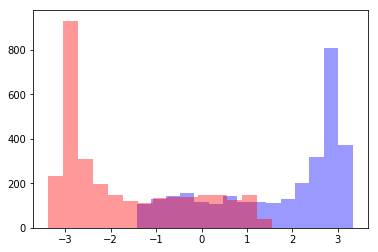
\includegraphics[width=1\linewidth]{img/wass_2moons_dist.png}
  \caption{Distribution of $\hat{f_c}$ conditionally to the classes}
  \label{wass:sub1}
\end{subfigure}%
\begin{subfigure}{.5\textwidth}
  \centering
  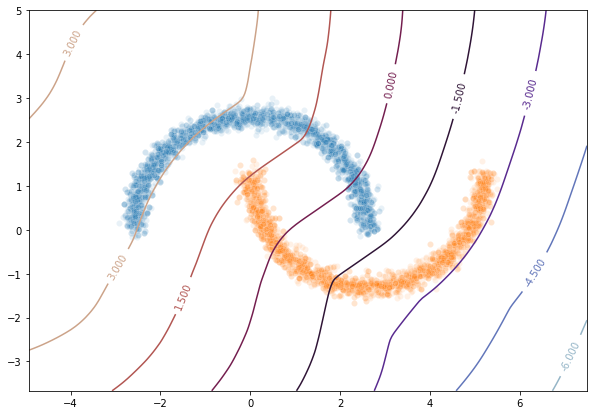
\includegraphics[width=1\linewidth]{img/wass_2moons_class.png}
  \caption{Level map of $\hat{f_c}$}
  \label{wass:sub2}
\end{subfigure}
\caption{Wasserstein classification (Eq.~\eqref{eq:wass_vanilla_classif}) on the two moons.}
\label{fig:wass}
\end{figure}





%%%%%%%%%%%%%%%%%%%%%%%%%%%%%%%%%%%%%%%%%%%%%%%%%%%%%%%%%%%%%%%%%%%%%%%%%%%%%%%%%%%%%%%%%%%%%%%%%%%%%%%%%%%%%%%%%%%%
\section{Hinge regularized Kantorovich-Rubinstein classifier }
\label{sec:kr_hinge}
%In this section we propose a regularized version of the Kantorovich-Rubinstein problem and we prove that it is still the dual of a transportation problem. Furthermore, we show that it has good properties in terms of robustness for classification problem.
\subsection{Definitions and primal transportation problem}
%\begin{figure}
%  \centering
%  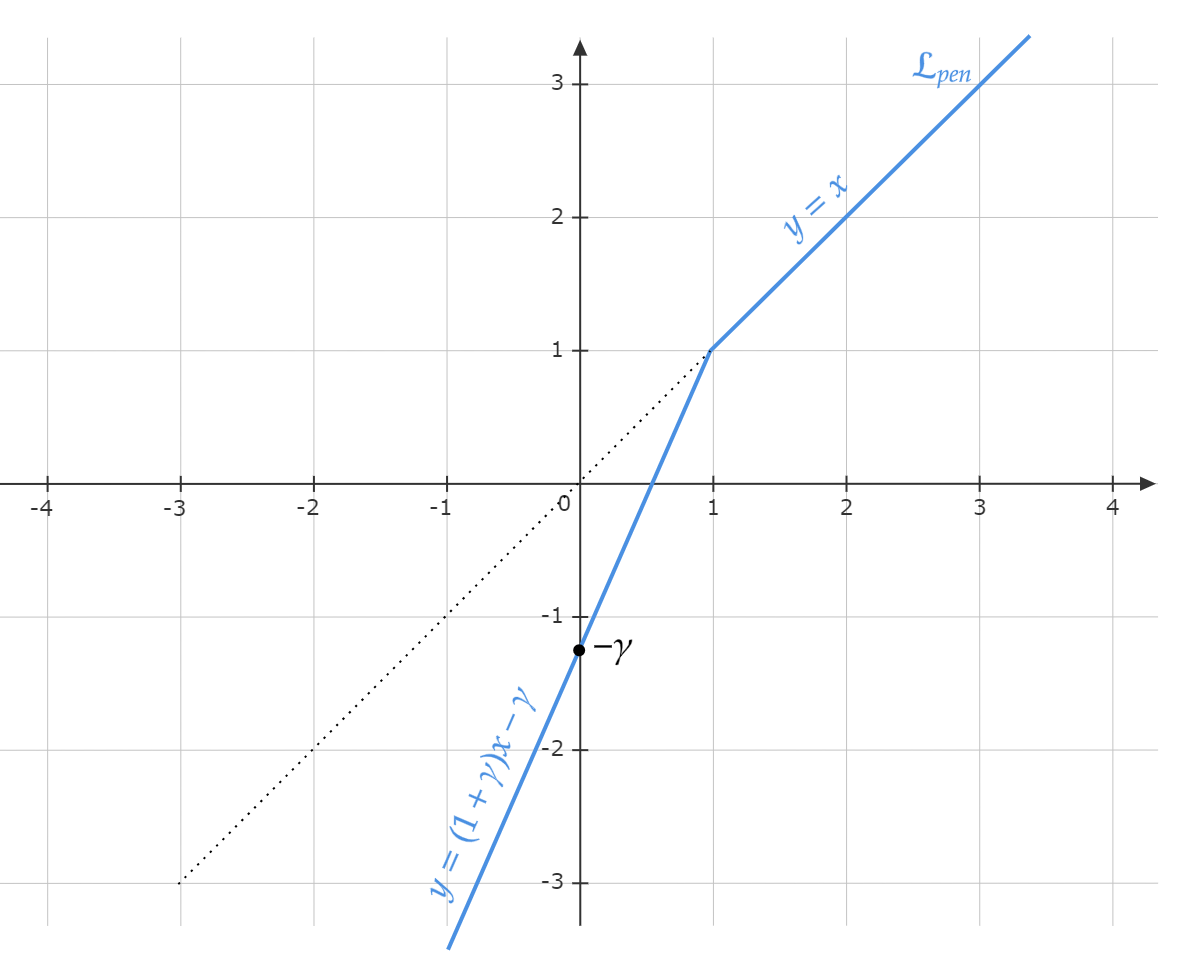
\includegraphics[width=0.7\linewidth]{img/loss_function.png}
%  \caption{$\mathcal{L}_{\W pen}$ loss function with respect to $yf(x)$.}
%  \label{fig:loss}
%\end{figure}%
In order to improve the classification abilities of the classifier based on Wasserstein distance, we propose a Kantorovich-Rubinstein optimization problem regularized by an hinge loss :
\begin{equation}
\label{eq:reg_OT}
\sup_{f \in Lip_1(\Omega)}-\mathcal{L}^{hKR}_\lambda(f)= \sup_{f \in Lip_1(\Omega)}-\left(\underset{\textbf{x}  \sim P_-}{\mathbb{E}} \left[f(\textbf{x})\right] -\underset{\textbf{x} \sim P_+}{\mathbb{E}}\left[f(\textbf{x})\right] +\lambda\underset{\textbf{x}}{\mathbb{E}} \left(1-Yf(\textbf{x})\right)_+\right)
\end{equation}
where $(1-\textbf{y}f(\textbf{x}))_+$ stands for the hinge loss $max(0,1-\textbf{y}f(\textbf{x}))$ and $\lambda>=0$. We name $\mathcal{L}^{hKR}_\lambda$ the hinge-KR loss. The goal is then to minimize this loss with an 1-Lipschitz neural network.

%we propose to replace the Wasserstein dual formulation, by the 
%of Wasserstein dual function, we propose the 
%following penalized version of Kantorovich-Rubinstein optimization problem that include an hinge loss:

When $\lambda=0$, this corresponds to the Kantorovich-Rubinstein dual optimization problem. Intuitively, the 1-Lipschitz function $f^*$ optimal with respect to Eq.~\eqref{eq:reg_OT} is the one that both separates the examples with a margin and spreads as much as possible the image of the distributions.
%{\color{red} (FRANCK: Cette phrase me parait inutile vu que c'est LIP1)It is obvious that, if the function $f$ is a neural network, this loss makes sense only if we constrain its Lipschitz constant. If not, $\W_{pen}$ will be infinite.} For misclassified or inside-margin samples the hinge-loss part is dominant, and the Kantorovich-Rubinstein part for the others samples. 
%The loss function behave like hinge-loss for miss-classified, or inside the margin examples example and like Kantorovich-Rubinstein function for the other. 


In the following, we introduce Theorems that prove the existence of such an optimal function $f^*$ and important properties of this function. Demonstrations of these theorems are in Appendix~\ref{appendix:proofs}.
\begin{Theorem} [Solution existence]
\label{Lemma:bounded_M}
 For each $\lambda>0$ there exists at least a solution $f^*$ to the problem  \[ f^*:=f_{\lambda}^*\in{\arg\min}_{f\in \text{Lip}_1(\Omega)}\mathcal{L}^{hKR}_{\lambda}(f) . \]
\end{Theorem}
Moreover, let $\psi$ be an optimal transport potential for the transport problem from $P_+$ to $ P_-$, $f^*$ satisfies that 
\begin{align}\label{eq:M}
	|| f^*||_{\infty}\leq M:= 1+\text{diam}(\Omega)+\frac{L_1(\psi)}{\inf(p,1-p)}.
\end{align}
%\footnote {{\color{red} (Franck) ne faudrait-il pas commenter l'apport de cette inégalité?  ?}}
The next theorem establishes that the Kantorovich-Rubinstein optimization problem with hinge regularization is still a transportation problem with relaxed constraints on the joint measure (which is no longer a joint probability measure).
\begin{Theorem}[Duality]\label{Theo:dual}
Set  $P_+, P_-\in \mathcal{P}(\Omega)$ and $\lambda>0$, then the following equality holds
\begin{align}\label{eq:dual}
\begin{split}
 \sup_{f\in \text{Lip}_1(\Omega)}- \mathcal{L}^{hKR}_\lambda(f)=	\inf_{\pi \in\Pi^p_{\lambda}(P_+, P_-)}\int_{\Omega\times \Omega}|{\textbf{x}}-{{\textbf{z}}} |d\pi + \pi_{\textbf{x}}(\Omega)+\pi_{{\textbf{z}}}(\Omega)-1
	\end{split}
\end{align}
Where $\Pi^p_{\lambda}(P_+, P_-)$ is the set consisting of positive measures $\pi\in \mathcal{M}_+(\Omega\times \Omega)$ which  are absolutely continuous with respect to the joint measure $dP_+\times dP_-$ and $\frac{d\pi_{\textbf{x}}}{dP_+}\in [p, p(1+\lambda)]$, $\frac{d\pi_{{\textbf{z}}}}{dP_-}\in [1-p, (1-p)(1+\lambda)] $.
%\footnote {{\color{red} (Franck) $[p, p(1+\lambda)]$ et $[1-p, (1-p)(1+\lambda)]$ me paraitrait plus clair}}
\end{Theorem}
%When the class are balanced, the constraints on $\pi$ became $\frac{d\pi_{\textbf{x}}}{d\mu}\in [\frac{1}{2}, \frac{1}{2}+\frac{1}{2}\lambda]$, $\frac{d\pi_{{\textbf{z}}}}{d\nu}\in [\frac{1}{2}, \frac{1}{2}+\frac{1}{2}\lambda] $ \footnote {{\color{red} (Franck) utile? obvious}}


\subsection{Classification and geometrical properties}
\label{sec:khr_properties}

\begin{figure}
\centering
\begin{subfigure}{.5\textwidth}
  \centering
  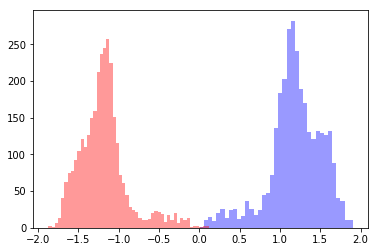
\includegraphics[width=1\linewidth]{img/wass_reg_2moons_dist.png}
  \caption{Distribution of $\hat{f}$ conditionally to the classes.}
  \label{wass_pen:sub1}
\end{subfigure}%
\begin{subfigure}{.5\textwidth}
  \centering
  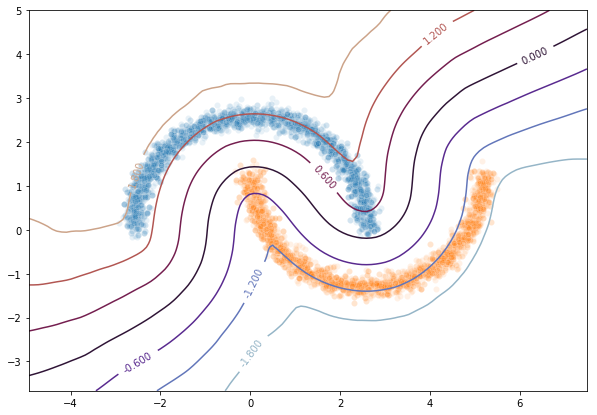
\includegraphics[width=1\linewidth]{img/wass_reg_2moons_class.png}
  \caption{Level map of $\hat{f}$}
  \label{wass_pen:sub2}
\end{subfigure}
\caption{Hinge regularized Kantorovich-Rubinstein (hinge-KR) classification on the two moons problem}
\label{fig:wass_pen}
\end{figure}
We note $\hat{f}$ the solution obtained by minimizing $\mathcal{L}^{hKR}_\lambda$ on a set of labeled examples and $f^*$ the solution of Eq.~\eqref{eq:reg_OT}. We don't assume that the solution found is optimal (i.e. $\hat{f}\neq f^*$) but we assume that $\hat{f}$ is 1-Lipschitz. Given a function $f$, a classifier based on $sign(f)$ and an example $x$, an adversarial example is defined as follows:
\begin{equation}
    adv(f,\textbf{x})=\underset{\textbf{z}\in \Omega | sign(f(\textbf{z}))=-sign(f(\textbf{x}))}{argmin}\parallel \textbf{x}-\textbf{z}\parallel.
\end{equation}
According to the 1-Lipschitz property of $\hat{f}$ we have 
\begin{equation}
\label{lowerbound}
%\parallel x- adv(\hat{f},x) \parallel \geq |\hat{f}(x)|.
|\hat{f}(\textbf{x})| \leq |\hat{f}(\textbf{x})-\hat{f}(adv(\hat{f},\textbf{x}))| \leq \parallel \textbf{x}- adv(\hat{f},\textbf{x}) \parallel.
\end{equation}
So $|\hat{f}(\textbf{x})|$ is a lower bound of the distance of $x$ to the separating boundary defined by $\hat{f}$ and thus a lower bound to the robustness to $l_2$ adversarial attacks. By minimizing $\mathbb{E} \left((1-\textbf{y}f(\textbf{x}))_+\right)$, we maximize the accuracy of the classifier and by maximizing the discrepancy of the image of $P_+$ and $P_-$ with respect to $f$ we maximize the robustness with respect to adversarial attack. The proposition below establishes that the gradient of the optimal function with respect to Eq.~\eqref{eq:reg_OT} has norm 1 almost surely, as for the unregularized case (Eq.~\eqref{eq:nabla_1}).
\begin{Proposition}\label{coro_norm1}
Let $\pi$ be the optimal measure of the dual version \eqref{eq:dual} of the hinge regularized optimal transport problem. Suppose that it is absolutely continuous with respect to Lebesgue measure. Then there exists at least a solution $f^*$ of \eqref{eq:dual} such that $||\nabla f^*||=1$ almost surely.
\end{Proposition}
 %Even we haven't prove it formally yet, empirical results suggest that given $\textbf{x}$, the image $tr_{f^*}(\textbf{x})$ of $\textbf{x}$ with respect to the transportation plan and $adv(\textbf{x})$ are in the same direction with respect to $x$ and this direction is $-f^*(\textbf{x})*\nabla_x f^*(\textbf{x})$ (i.e $adv(\textbf{x})\approx x-c_x*f^*(\textbf{x})*\nabla_x f^*(\textbf{x})$ and $tr_{f^*}(\textbf{x})\approx x-c'_x*f^*(\textbf{x})*\nabla_x f^*(\textbf{x})$ with $0 \leq c_x \leq c_x' \in \mathbb{R} $). This would link the adversarial attack to the optimal transport.
Furthermore, empirical results suggest that given $\textbf{x}$, the image $tr_{f^*}(\textbf{x})$ of $\textbf{x}$ with respect to the transportation plan and $adv(\textbf{x})$ are in the same direction with respect to $\textbf{x}$ and the direction is % and 
 $-\nabla_x f^*(\textbf{x})$. Combining this direction with the Eq.~\eqref{lowerbound}, we will show empirically (sect.~\ref{sec:experimentation}) that  $$adv(\textbf{x})\approx x-c_x*f^*(\textbf{x})*\nabla_x f^*(\textbf{x})$$ and $$tr_{f^*}(\textbf{x})\approx x-c'_x*f^*(\textbf{x})*\nabla_x f^*(\textbf{x})$$ with $1 \leq c_x \leq c_x' \in \mathbb{R} $. This provides a strong link between the adversarial attack and the optimal transport for the proposed classifier.
 
 
The next proposition shows that, if the classes are well separated, maximizing the hinge-KR loss leads to a perfect classifier.% with no error.
\begin{Proposition}[Separable classes]\label{coro:epsilon}
Set  $P_+, P_-\in \mathcal{P}(\Omega)$ such that $P(Y=+1)=P(Y=-1)$ and $\lambda\geq 0$ and suppose that there exists $\epsilon>0$ such that
\begin{align}\label{coro:hipotesis}
	| {\textbf{x}}-{\textbf{{{\textbf{z}}}}} |> 2 \epsilon \ \ dP_+\times dP_- \text{ almost surely}
\end{align}
Then for each
\begin{align}
	f_{\lambda}\in {\arg\sup}_{f\in \text{Lip}_{1/\epsilon}(\Omega)}\int_{\Omega}f(dP_+-dP_-)-\lambda \left( \int_{\Omega}(1-f)_+dP_+ +\int_{\Omega}(1+f)_+dP_-\right),
\end{align}
it is satisfied that $L_1(f_{\lambda})=0.$ Furthermore if $\epsilon\geq 1$ then $f_{\lambda}$ is an optimal transport potential from $P_+$ to $P_-$ for the cost $| {\textbf{x}}-{{\textbf{z}}}|$.
\end{Proposition}
We show in Fig.~\ref{fig:wass_pen}, on the two moons problem, that in contrast to the vanilla classifier based on Wasserstein (Eq.~\eqref{eq:wass_vanilla_classif}), the proposed approach enables non overlapping distributions of $\hat{f}$ conditionally to the classes (Fig.~\ref{wass_pen:sub1}).
%Figure~\ref{fig:wass_pen} illustrates the approach on the two moons problem. Contrarily to the example with Wasserstein, we observe that the distributions of $f$ conditionally to the classes doesn't overlap (Figure~\ref{wass_pen:sub1}). 
In the same way, the 0-level cut of $\hat{f}$ (Fig.~\ref{wass_pen:sub2}) is a nearly optimal classification boundary. Moreover, the level cut of $\hat{f}$, on the support of the distributions, is close to the distance to this classification boundary.
%, corresponds approximately to the distance to the classification boundary.  

\section{1-Lipschitz neural networks}
\label{sec:lip_const}
In order to build a deep learning classifier based on the hinge-KR optimization problem (Eq.~\eqref{eq:reg_OT}), we have to constrain the Lipschitz constant of the neural network to be equal to 1. Even if the control of the Lipschitz constant of a neural network is a key step to guarantee some robustness \cite{cisse_parseval_2017}, it is known that evaluating it exactly is a np-hard problem~\cite{NIPS2018_7640}. The simplest strategy is to constraint each layer of the network to be 1-Lipschitz, to ensure that the Lipschitz constant of composition of the functions will be less than or equal to one. Most common activation functions such as ReLU or sigmoid are 1-Lipschitz. In the case of a dense layer, constraints can be applied to its weights. 
The simplest strategy is to constraint the weights of each layer.  Given a dense layer with weights $W$, 
It is commonly admitted that:
\begin{equation}
\label{norm_mat}
    L(W)=||W|| \leq ||W ||_F \leq \underset{ij}{max}(|W_{ij}|)*\sqrt{nm}
\end{equation}
where $|| W||$ is the spectral norm, and  $|| W||_F$ is the Frobenius norm.
The initial version of WGAN \cite{Arjovsky2017} consisted of clipping the weights of the networks. However, this is a very crude way to upper-bound Lipschitz constant (last term in Eq.~\eqref{norm_mat}).
Normalizing by the Frobenius norm has also been proposed in~\cite{SalimansK16}. In this paper, we use spectral normalization as proposed in \cite{Miyato2018SpectralNF}, since the spectral norm is equals to the Lipschitz constant. At the inference step, we normalize the weights of each layer by dividing the weights by the spectral norm of the matrix. The spectral norm is computed by iteratively evaluating the largest singular value with the power iteration algorithm~\cite{GOLUB200035}. This is done during the forward step and taken into account for the gradient computation.\\

In the case of 2D-convolutional layers, normalizing by the spectral norm of the convolution kernels is not enough and a supplementary multiplicative constant $\Lambda$ is required (the regularization is then done by dividing $W$ by $\Lambda||W||$). Given a convolutional layer with a kernel size equals to $k=2*\bar{k}+1$, the coefficient $\Lambda$ can be estimated, as in~\cite{cisse_parseval_2017}, as the square root of the maximum number of duplications of the input matrix values: since each input can be used in at most $k^2$ positions, choosing $\Lambda=k$ guarantees the convolutional layers to be 1-Lipschitz. However, due to the effect of the zero-padding, the constant $\Lambda$ is overestimated and the real Lipschitz constant is lower than 1, especially when the size of the image is small. When the convolutional network is very deep, this heavily decreases  the Lipschitz constant of the neural network. To mitigate this effect, we propose, for zero padding, a tighter estimation of $\Lambda$, computing the average duplication factor of non zero padded values in the feature map:
\begin{equation}
\Lambda=\sqrt{\frac{(k.w-\bar{k}.(\bar{k}+1)).(k.h-\bar{k}.(\bar{k}+1))}{h.w}}.
\label{eq:ConvApproxLip}
\end{equation}
Even if this constant doesn't provide a strict upper bound of the Lipschitz constant (for instance, when the higher values are located in the center of the picture), it behaves very well empirically (see Figure \ref{fig:l2_norm_VGG_wass} for instance).
%\footnote{{\color{red} (FRANCK:il me semble que la phrase est un peu légère, ou alors faire une ref aux experiments et la figure 3???}}. 
Convolution with stride, pooling layers, detailed explanations and demonstrations are discussed in Appendix~\ref{sec:convStride}.\\

As shown in Section~\ref{sec:khr_properties}, the optimal function $f^*$ with respect to Eq.~\eqref{eq:reg_OT}, verifies $||\nabla f^* ||=1$ almost surely.
In \cite{gulrajani2017improved}, the authors propose to add a regularization term with respect to the average gradient norm with respect to inputs in the loss function. However, the estimation of this value is difficult and a regularization term doesn't guarantee the property. In this paper, we apply the approach described in \cite{pmlr-v97-anil19a}, based on the use of specific activation functions and a process of normalization  of the weights. Two norm preserving activation functions are proposed: i)\ \textbf{GroupSort2} : order the vector by pairs, ii) \textbf{FullSort} : order the full vector.
These functions are vector-wise rather than element-wise. We also use the P-norm pooling \cite{boureau2010},with $P=2$ which is a norm-preserving average pooling.
%We also propose the activation  \textbf{ConstPReLU}, a PReLU \cite{He_2015} activation function complemented by a constraint such that $|\alpha|\leq 1$ ($\alpha$ the learned slope). This last function is norm preserving only when $|\alpha|=1$ (linear, or absolute value function), but being computed element wise, it is more efficient for convolutional layers outputs.
Concerning linear functions, a weight matrix $W$ is norm preserving if and only if all the singular values of $W$ are equals to $1$. In \cite{pmlr-v97-anil19a}, the authors propose to use the Björck orthonormalization algorithm \cite{bjorck71Ortho}. This algorithm is fully differential and, as for spectral normalization, is applied during the forward inference, and taken into account for back-propagation (see Appendix~\ref{app:normpreserving} for details). We also developed a full tensorflow~\cite{tensorflow2015-whitepaper} implementation in an opensource library, called \Deellip, that enables training of k-Lipschitz neural networks, and exporting them as standard layers for inference. 








%%%%%%%%%%%%%%%%%%%%%%%%%%%%%%%%%%%%%%%%%%%%%%%%%%%%%%%%%%%%%%%%%%%%%%%%%%%%%%%%%%%%%%%%%


\section{Experiments}
\label{sec:experimentation}
In the experiment, we compare three different approaches: i) classical log-entropy classifier (MLP/CNN), ii) 1-Lipschitz log-entropy classifier (1LIP-MLP/1LIP-CNN), in the spirit of Parseval networks, iii) hinge-KR classifier (hKR-MLP/hKR-CNN). In order to have a fair comparison, all the classifiers share the same dense or convolutional architecture. 
% For the 1-Lipschitz layer we have developed the open source library DEELLIP. 
For the 1-Lipschitz log-entropy, we perform spectral normalization within the experiments with 3 power iteration steps and we use ReLU activation (gradient preserving activations and pooling make no sense in this case and Björck orthonormalization doesn't improve the results). For the hinge-KR classifiers, we apply Björck orthonormalization (15 steps with p=1) after the spectral normalization (this improves the convergence of the Björck algorithm). We use fullsort activation for dense layers and GroupSort2 for the convolutional ones. The full description of the architecture, the optimization process, and the influence of each parameter are described in Appendix~\ref{sec:networks_architecture}. 

For adversarial robustness estimation, since the hinge-KR primal problem is linked to $L_2$ distance, we focus on $L_2$ based adversarial attacks using the \textit{DeepFool} framework~\cite{moosavi-deepfool15}. For each type of Neural Network, 500 attacks are carried out on test sets (using the \textit{foolbox} library~\cite{rauber_foolbox_2018}), storing for each image the $output$ value, and the $L_2$ norm of noise  required to fool the network (up to a 50/50 score). The $output$ value is either the last dense layer output before the sigmo\"id activation for MLP/CNN and 1LIP-MLP/1LIP-CNN networks (commonly called $logit$ layer), or the last layer output for the hKR-MLP/hKR-CNN classifier. %Classically, to be compatible with \textit{foolbox}, a two outputs network is provided with $(logit,-logit)$ values.
We consider two binary classification problems. The first one is the separation of the digits 0 and 8 on the MNIST dataset (balanced classes, 10596 training, and 1954 test samples). We choose these particular pair of digits because they are the hardest to separate. In the second problem, we consider the separation between male people with or without mustaches on the CelebA dataset \cite{liu2015faceattributes} (unbalanced classes, 11779 training ($36\%$ with mustache), 11036 test samples ($37\%$) ).


%\subsection{Regularized optimal transport classifier accuracy and rejection rule}
%\label{sec:hinge-KR-accuracy}
%NDLR: voir si les expe TwoMoons doivent être mises ici ou pas 


 Table~\ref{tab:acc_comparison} compares the classification accuracy and the adversarial robustness results for the three types of classifiers.  The drop in accuracy for the proposed solution, compared to classical networks, is less than one point even for a complex task such as celeb-A moustache classification. The last column of the table compares the average $L_2$ norm of adversarial noise for the three types of classifier. On the MNIST dataset, the improvement of robustness with 1-Lipschitz layers is significant with a clear advantage for our approach. When considering the CelebA problem, using 1-Lipschitz layers with log-entropy is not enough (the $logit$ values tend to be small). The proposed hKR approach leads to a classifier that is up to 10 times more robust than its competitors with an acceptable loss of accuracy.
 
\begin{table}[]
    \centering
    \begin{tabular}{|c|c|c|c|c|c|}
    \hline
       Dataset  & \shortstack{Network \\archi}  & loss & Accuracy & \shortstack{Attack\\ Robustness}\\ \hline
       \multirow{5}{*}{MNIST 0-8} & $MLP$  & bin\_cross. & 99.6 & 4.47 \\
        & $1LIP-MLP$   &  bin\_cross. & 99.5 & 6.29  \\
        & $hKR-MLP$ &  $L^{hKR}_\lambda$ ($\lambda=10$) & 99.0  & 7.19 \\
        & $hKR-MLP$ &   $L^{hKR}_\lambda$ ($\lambda=50$) & 99.2 & \textbf{7.36}  \\\hline
       \multirow{3}{*}{\shortstack{Celeb-A \\Moustache} }  & $CNN$ & bin\_cross. & 92.6& 0.45  \\
       & $1LIP-CNN$  &  bin\_cross. & 92.4 & 0.27  \\
       & $hKR-CNN$  & $L^{hKR}_\lambda$ ($\lambda=20$)  & 90.9  & \textbf{3.87 }\\\hline
    \end{tabular}
    \caption{Accuracy and robustness to adversarial attack (average noise $L_2$ norm) comparison}
    \label{tab:acc_comparison}
\end{table}

%\subsection{Robustness evaluation and interpretation}
%\label{sec:Hinge-KR-robustness}

In Fig.~\ref{fig:l2norm_vs_logit}, we compare, on the MNIST 0-8 dataset, the $L_2$ norm of adversarial samples with respect to the output of the hKR neural networks (and the logit values for the 1LIP network). Figures~\ref{fig:l2norm_MLP_wass} and~\ref{fig:l2_norm_VGG_wass}  show that with our proposed learning rule, the fooling noise for a given input is linearly linked to the output (slope of one for MLP,  and around 1.1 for CNN), which confirms that the Lipschitz constants of our networks are very close to (but lower than) 1.
We also observe that, for a given input sample, the network prediction represents a very tight lower bound of the adversarial robustness of the network for this sample. In contrast, for the 1LIP-MLP (Fig.~\ref{fig:l2_norm_MLP_lipsigmoid}), the 1-Lipschitz constraint is also guaranteed, but the output of the network can be far lower than the adversarial noise norm.%\footnote{{\color{red} (FRANCK) je ne comprend pas la phrase) MAthieu (j'avois oublié des mots :)}}
While on some samples at the tail end of the distribution, the  $L_2$ norm of found noise can reach 30, the average adversarial robustness is lower  than for the proposed solution (green vertical lines).
%\footnote{{\color{red} (FRANCK) j'ai changé la phrase sur les conseil de Doug pour une meilleure comprehension. A verifier}}
%While on some samples, the  $L_2$ norm of found noise can reach 30, the average adversarial robustness is lower (green vertical lines), and high noise values are only for some points at the tail end of the distribution. 
Beside the level of noise, Figures~\ref{fig:Deep_fool_MNIST08} empirically show that, in contrast to the other approaches, the noise required to change the output class for the hKR classifier is highly structured, and interpretable. Thus, on the MNIST 0-8 dataset, in order to fool the proposed  learned network with \textit{DeepFool}, a 0-image, for instance, is explicitly transformed into a mix between an 8 and a 0. Even for a more complex task, such as a mustache classifier on the Celeb-A dataset, Fig.~\ref{fig:Deep_fool_CelebA} shows that fooling an image of a male without (resp. with) a mustache requires to addition (resp. removal) of dark pixels around the nasolabial fold. We also build counterfactual examples (line d) by applying the scheme proposed in Section \ref{sec:khr_properties}  (i.e. $counter(\hat{f},\textbf{x})\approx x-c_x*\hat{f}(\textbf{x})*\nabla_x \hat{f}(\textbf{x})$). For each sample, we choose $c_x$ to obtain a visually satisfactory counterfactual (and not at the classification boundary as for adversarial examples). Although the differential images are not as precise as the ones obtained with adversarial approach, they clearly focus on the meaningful part of the images and provide, in our opinion, convincing counterfactual explanations. Remark that this approach is closely related to saliency map. However, the results obtained with our network are far more precise than the ones on classical networks.   %\footnote{{\color{red} (FRANCK) est ce qu'on rajoute et inversement, ou ce n'est pas assez visible? MAthieu modifié, dis moi  si c'est ok}}

%[besoin de plus d'arguments+ peut etre la même chose sur CelebA]



\begin{figure}
\centering
\begin{subfigure}{.3\textwidth}
  \centering
  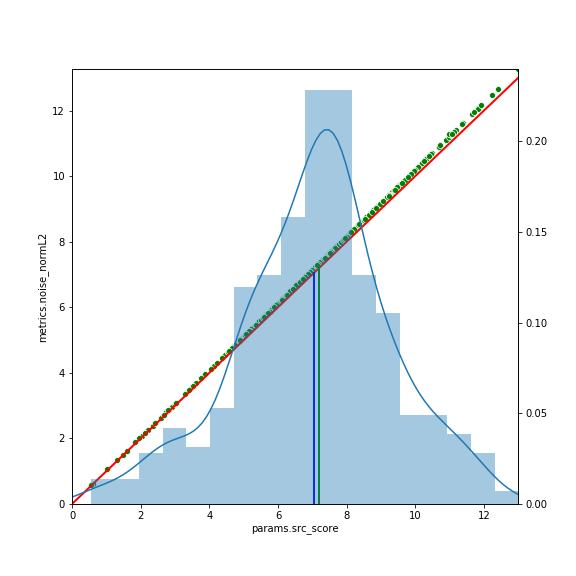
\includegraphics[width=1\linewidth]{img/deepfool_vs_score_DeepFool_Regularized_OT_MLP_new.png}
  \caption{hKR-MLP}
  \label{fig:l2norm_MLP_wass}
\end{subfigure}%
\begin{subfigure}{.3\textwidth}
  \centering
  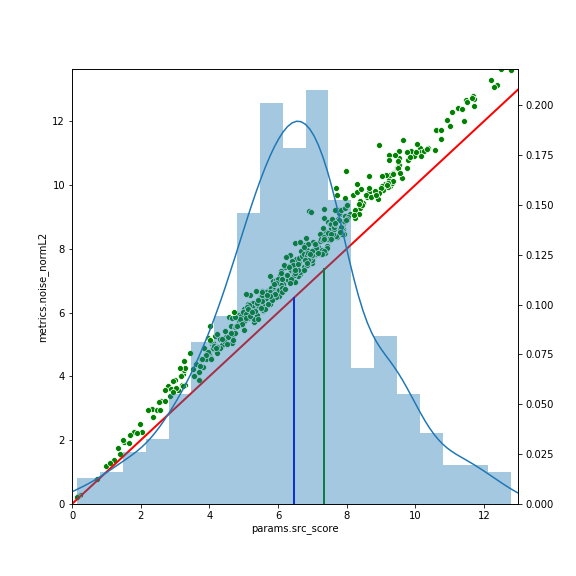
\includegraphics[width=1\linewidth]{img/deepfool_vs_score_DeepFool_Regularized_OT_VGG_new.png}
  \caption{hKR-CNN}
  \label{fig:l2_norm_VGG_wass}
\end{subfigure}
\begin{subfigure}{.3\textwidth}
  \centering
  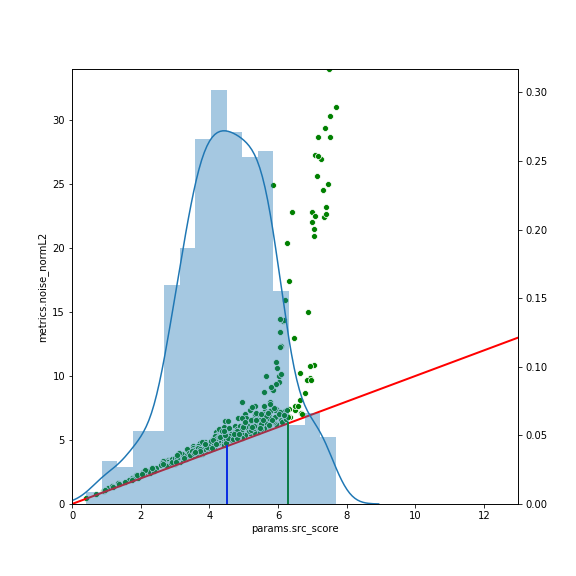
\includegraphics[width=1\linewidth]{img/deepfool_vs_score_DeepFool_Lipschitz_Sigmoid_new.png}
  \caption{1LIP-CNN}
  \label{fig:l2_norm_MLP_lipsigmoid}
\end{subfigure}
\caption{Comparison of $L_2$ norm of fooling noise (Y-axis) with the $output$ value (X-axis): green dots noise norm for samples (green line average value), red line:  minimal possible noise (1-lipschitz), blue histogram: $output$ (resp. $logit$ for 1LIP-CNN) distribution (blue line average value)
}
\label{fig:l2norm_vs_logit}
\end{figure}
 

\begin{figure}
\centering
\begin{subfigure}{1\textwidth}
  \centering
  
\includegraphics[width=0.24\linewidth]{img/fooling/model_MLP128_sigmoid_ReLU_src_and_adv_22.png}
  
\includegraphics[width=0.24\linewidth]{img/fooling/model_MLP128_sigmoid_ReLU_src_and_adv_34.png}
  
\includegraphics[width=0.24\linewidth]{img/fooling/model_MLP128_sigmoid_ReLU_src_and_adv_42.png}
  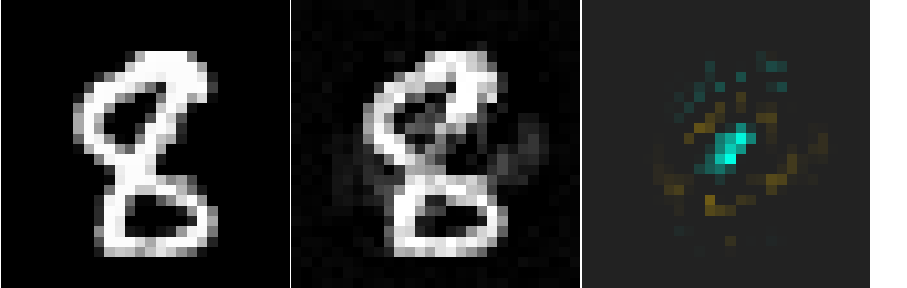
\includegraphics[width=0.24\linewidth]{img/fooling/model_MLP128_sigmoid_ReLU_src_and_adv_56.png}
  \caption{MLP with sigmo\"id and binary cross entropy}
\end{subfigure}
\begin{subfigure}{1\textwidth}
  \centering
  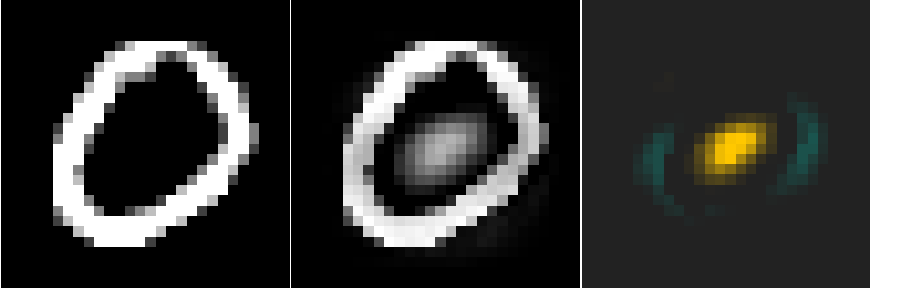
\includegraphics[width=0.24\linewidth]{img/fooling/model_MLP_Lip_Sigmoid_src_and_adv_22.png}
  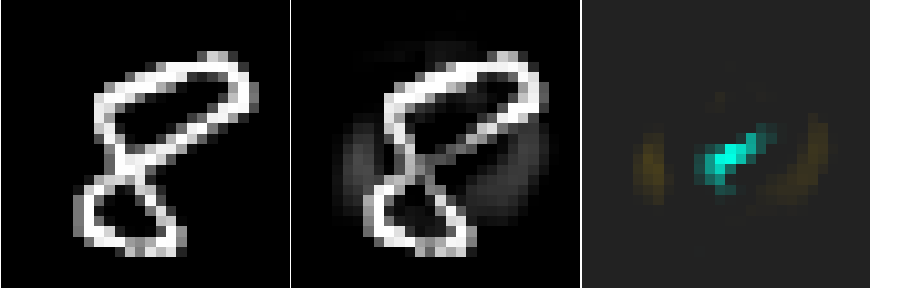
\includegraphics[width=0.24\linewidth]{img/fooling/model_MLP_Lip_Sigmoid_src_and_adv_34.png}
  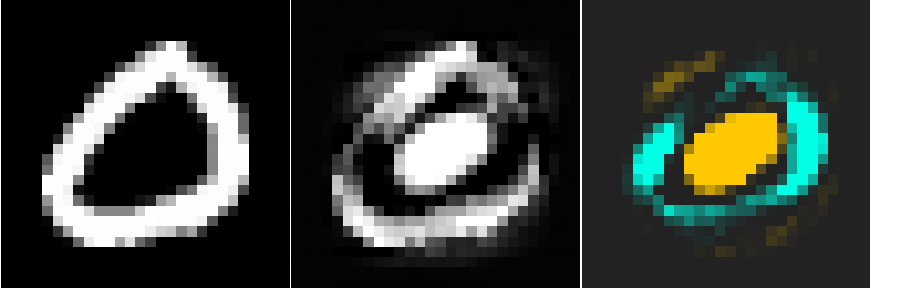
\includegraphics[width=0.24\linewidth]{img/fooling/model_MLP_Lip_Sigmoid_src_and_adv_42.png}
  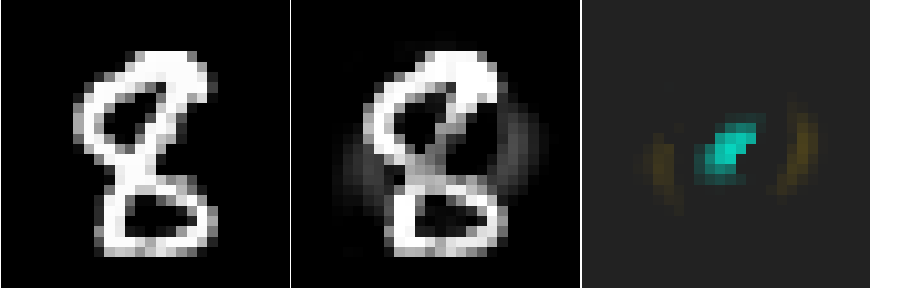
\includegraphics[width=0.24\linewidth]{img/fooling/model_MLP_Lip_Sigmoid_src_and_adv_56.png}
  \caption{MLP Lipschitz with sigmo\"id and binary cross entropy}
\end{subfigure}
\begin{subfigure}{1\textwidth}
  \centering
  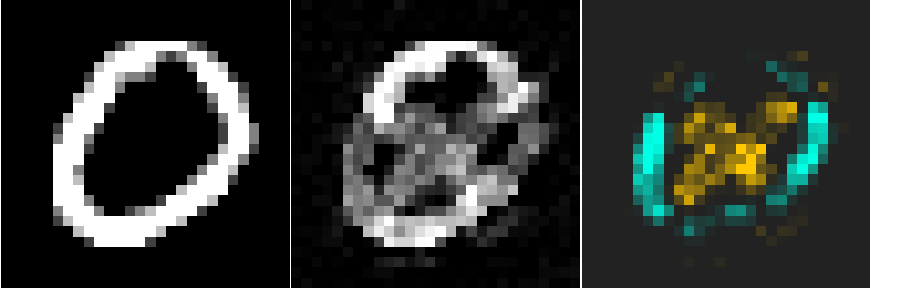
\includegraphics[width=0.24\linewidth]{img/fooling/model_MLP_Bjorck_FullSort_hKR_src_and_adv_22.png}
  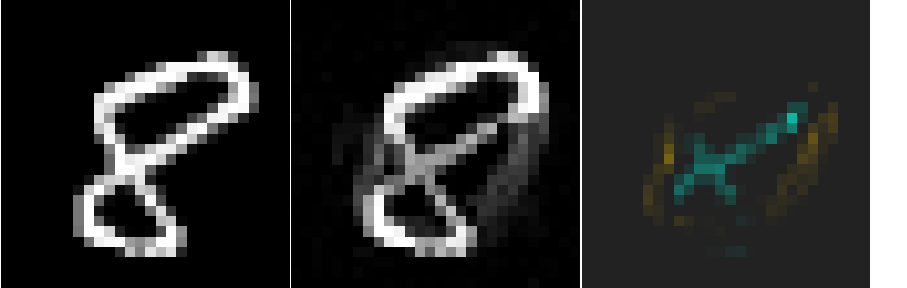
\includegraphics[width=0.24\linewidth]{img/fooling/model_MLP_Bjorck_FullSort_hKR_src_and_adv_34.png}
  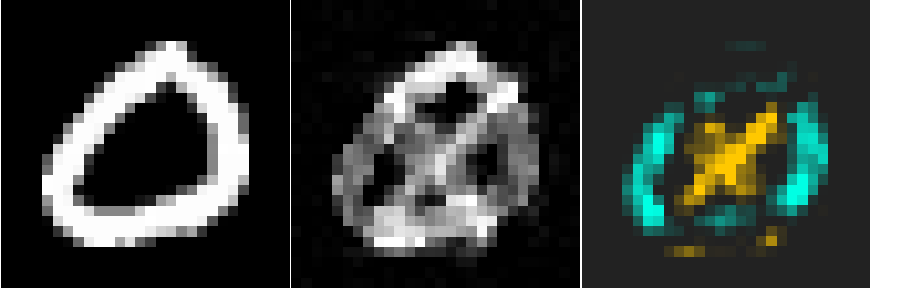
\includegraphics[width=0.24\linewidth]{img/fooling/model_MLP_Bjorck_FullSort_hKR_src_and_adv_42.png}
  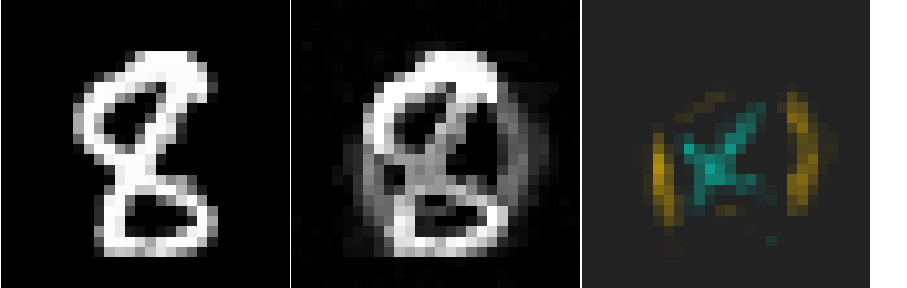
\includegraphics[width=0.24\linewidth]{img/fooling/model_MLP_Bjorck_FullSort_hKR_src_and_adv_56.png}
  \caption{MLP Lipschitz with the proposed hinge-KR loss}
\end{subfigure}


\caption{Deepfool adversarial examples on MNIST 0-8 dataset: source image, fooled image, differential image (yellow (resp. cyan) increase(resp. decrease) grey level)}
\label{fig:Deep_fool_MNIST08}
\end{figure}


% \begin{figure}
% \centering
% \begin{subfigure}{1.\textwidth}
% \begin{subfigure}{.5\textwidth}
%   \centering
%   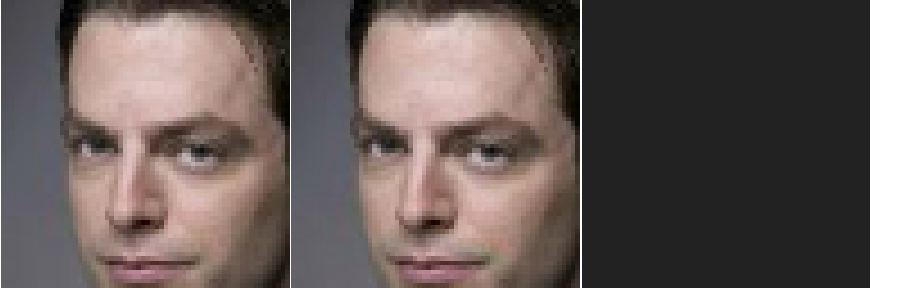
\includegraphics[width=1\linewidth]{img/fooling/AddingMoustache_35_Classic.png}
%   \label{fig:AddingMoustache_35_Classical}
% \end{subfigure}%
% \begin{subfigure}{.5\textwidth}
%   \centering
%   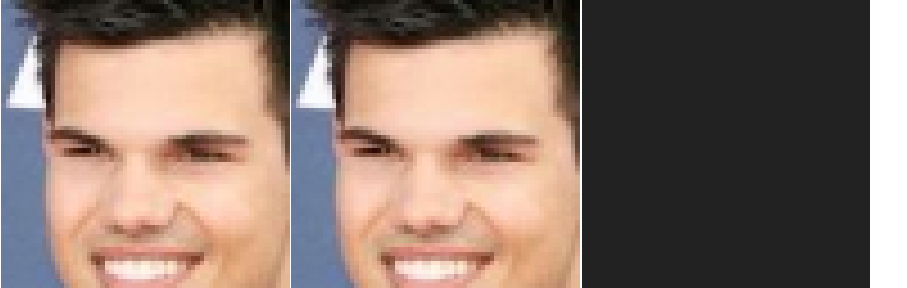
\includegraphics[width=1\linewidth]{img/fooling/AddingMoustache_58_Classic.png}
%   \label{fig:AddingMoustache_58_Classical}
% \end{subfigure}  
% \caption{Fooling "non-moustache" images classical network}
% \end{subfigure}  
% \begin{subfigure}{1.\textwidth}
% \begin{subfigure}{.5\textwidth}
%   \centering
%   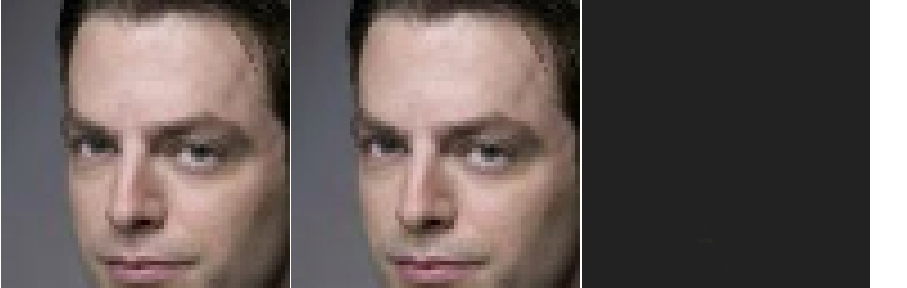
\includegraphics[width=1\linewidth]{img/fooling/AddingMoustache_35_1LipSigmoid.png}
%   \label{fig:AddingMoustache_35_Lip_binCross}
% \end{subfigure}%
% \begin{subfigure}{.5\textwidth}
%   \centering
%   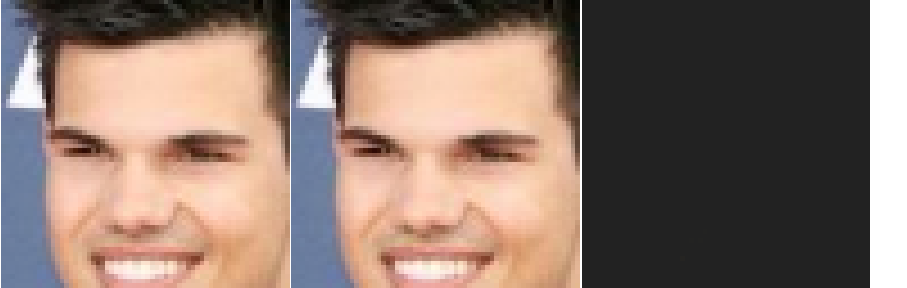
\includegraphics[width=1\linewidth]{img/fooling/AddingMoustache_58_1LipSigmoid.png}
%   \label{fig:AddingMoustache_58_Lip_binCross}
% \end{subfigure}  
% \caption{Fooling "non-moustache" images 1-lipschitz network (binary crossentropy)}
% \end{subfigure}  
% \begin{subfigure}{1.\textwidth}
% \begin{subfigure}{.5\textwidth}
%   \centering
%   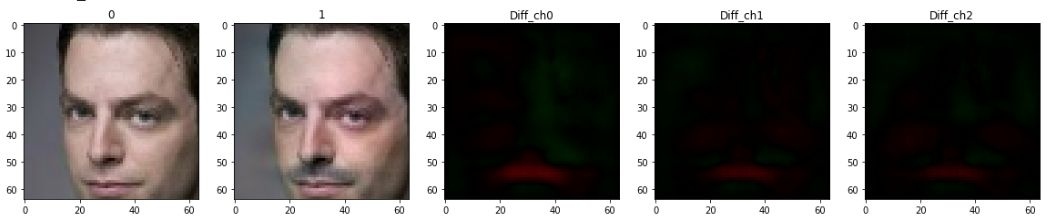
\includegraphics[width=1\linewidth]{img/AddingMoustache_1_OK.jpg}
%   \label{fig:AddingMoustache_1_OK}
% \end{subfigure}%
% \begin{subfigure}{.5\textwidth}
%   \centering
%   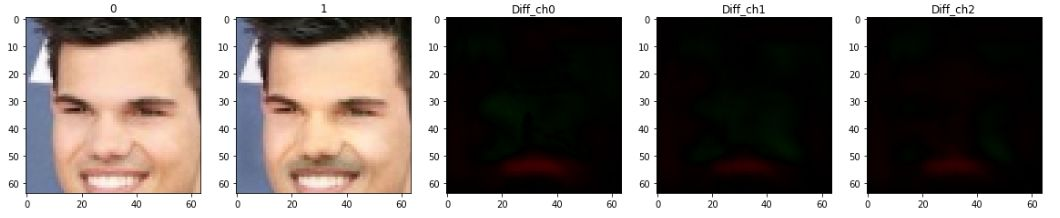
\includegraphics[width=1\linewidth]{img/AddingMoustache_5_OK.jpg}
%   \label{fig:AddingMoustache_5_OK}
% \end{subfigure}
% \begin{subfigure}{.5\textwidth}
%   \centering
%   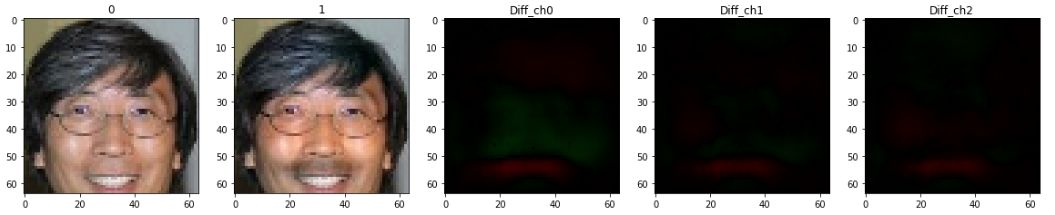
\includegraphics[width=1\linewidth]{img/AddingMoustache_4_OK.jpg}
%   \label{fig:AddingMoustache_3_OK}
% \end{subfigure}%
% \begin{subfigure}{.5\textwidth}
%   \centering
%   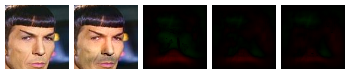
\includegraphics[width=1\linewidth]{img/AddingMoustache_218_OK.png}
%   \label{fig:AddingMoustache_4_OK}
% \end{subfigure}
% \caption{Fooling "non-moustache" images with the proposed Hinge-KR classifier}
% \end{subfigure}  
% \begin{subfigure}{1.\textwidth}
% \begin{subfigure}{.5\textwidth}
%   \centering
%   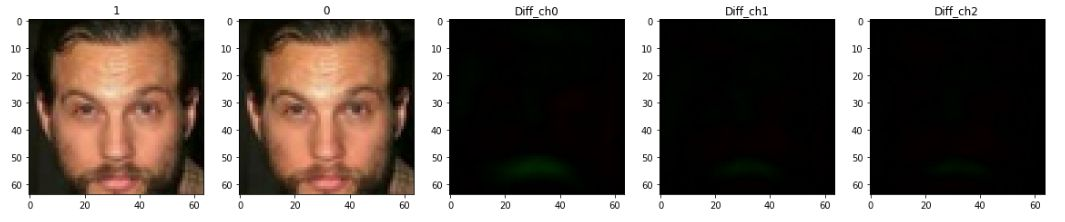
\includegraphics[width=1\linewidth]{img/RemovingMoustache_4_OK.jpg}
%   \label{fig:RemovingMoustache_4_OK}
% \end{subfigure}%
% \begin{subfigure}{.5\textwidth}
%   \centering
%   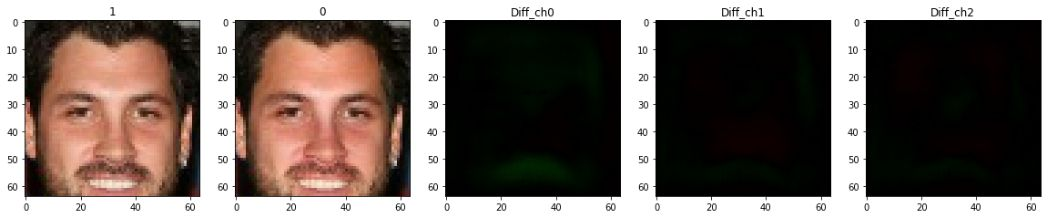
\includegraphics[width=1\linewidth]{img/RemovingMoustache_2_OK.jpg}
%   \label{fig:RemovingMoustache_2_OK}
% \end{subfigure}
% \begin{subfigure}{.5\textwidth}
%   \centering
%   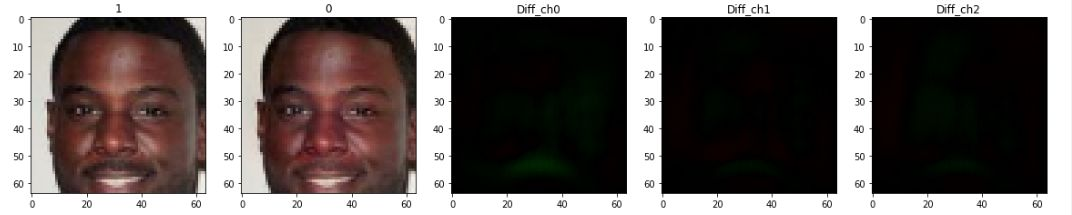
\includegraphics[width=1\linewidth]{img/RemovingMoustache_5_OK.jpg}
%   \label{fig:RemovingMoustache_5_OK}
% \end{subfigure}%
% \begin{subfigure}{.5\textwidth}
%   \centering
%   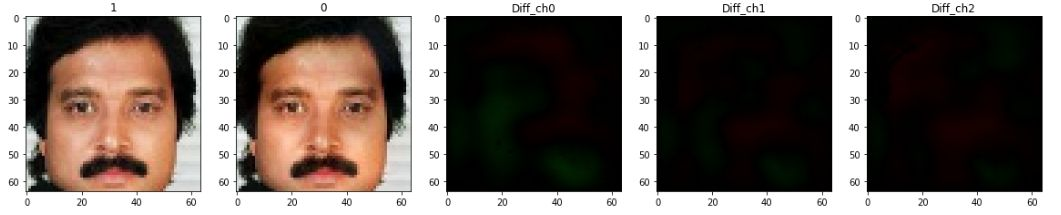
\includegraphics[width=1\linewidth]{img/RemovingMoustache_1_KO.jpg}
%   \label{fig:RemovingMoustache_1_KO}
% \end{subfigure}
%   \caption{Fooling "moustache" images with the proposed Hinge-KR classifier}
% \end{subfigure}  
% \caption{Deepfool adversarial examples  on Celeb-A dataset. Classical networks and 1-lipschitz networks learned with binary crossentropy lead to invisble noise, whereas proposed solution add or remove dark pixels around the nasolabial fold}
% \label{fig:Deep_fool_CelebA}
% \end{figure}
 
%\begin{figure}
%\centering
%\begin{subfigure}{1.\textwidth}
%    \begin{subfigure}{.25\textwidth}
%      \centering
%%      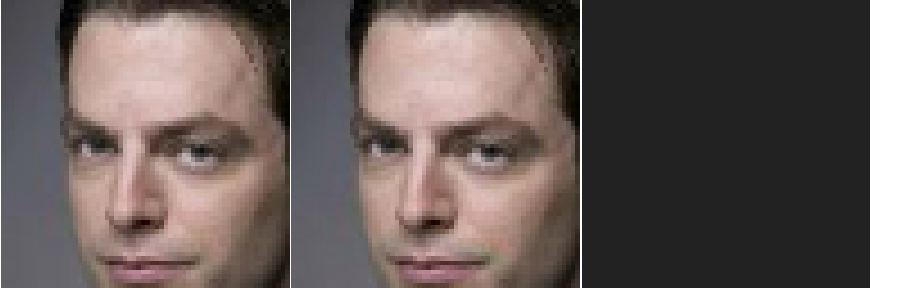
\includegraphics[width=1\linewidth]{img/fooling/AddingMoustache_35_Classic.png}
%      \label{fig:AddingMoustache_35_Classical}
%    \end{subfigure}%
%    \begin{subfigure}{.25\textwidth}
%      \centering
%      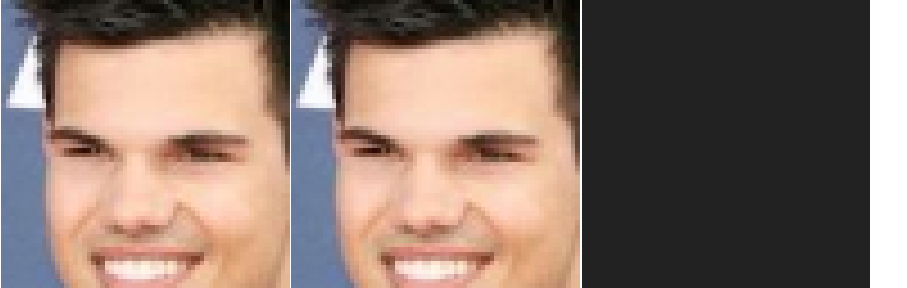
\includegraphics[width=1\linewidth]{img/fooling/AddingMoustache_58_Classic.png}
%      \label{fig:AddingMoustache_58_Classical}
%    \end{subfigure}  
%    \begin{subfigure}{.25\textwidth}
%      \centering
%      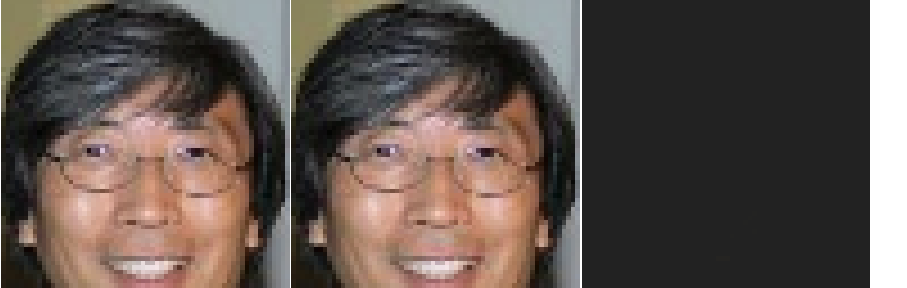
\includegraphics[width=1\linewidth]{img/fooling/AddingMoustache_54_Classic.png}
%      \label{fig:AddingMoustache_58_Lip_binCross}
%    \end{subfigure}  
%    \caption{Fooling "non-moustache" images classical network}
%\end{subfigure}  
%\begin{subfigure}{1.\textwidth}
%    \begin{subfigure}{.25\textwidth}
%      \centering
%      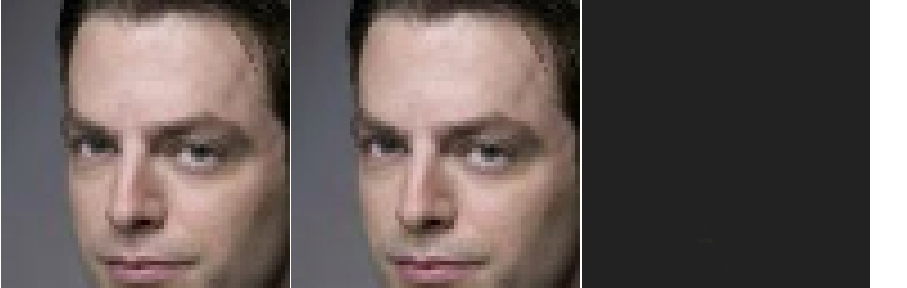
\includegraphics[width=1\linewidth]{img/fooling/AddingMoustache_35_1LipSigmoid.png}
%      \label{fig:AddingMoustache_35_Lip_binCross}
%    \end{subfigure}%
%    \begin{subfigure}{.25\textwidth}
%      \centering
%      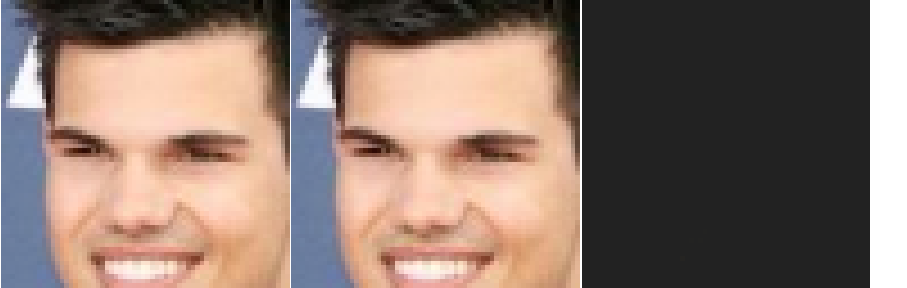
\includegraphics[width=1\linewidth]{img/fooling/AddingMoustache_58_1LipSigmoid.png}
%      \label{fig:AddingMoustache_58_Lip_binCross}
%    \end{subfigure} 
%    \begin{subfigure}{.25\textwidth}
%      \centering
%      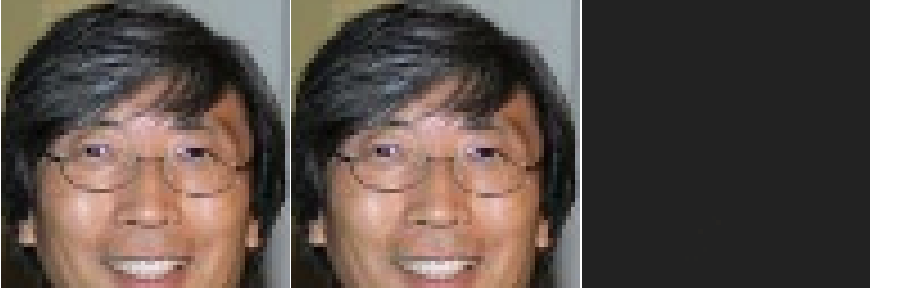
\includegraphics[width=1\linewidth]{img/fooling/AddingMoustache_54_1LipSigmoid.png}
%      \label{fig:AddingMoustache_58_Lip_binCross}
%    \end{subfigure}  
%    \caption{Fooling "non-moustache" images 1-lipschitz network (binary crossentropy)}
%\end{subfigure}  
%\begin{subfigure}{1.\textwidth}
%    \begin{subfigure}{.25\textwidth}
%      \centering
%      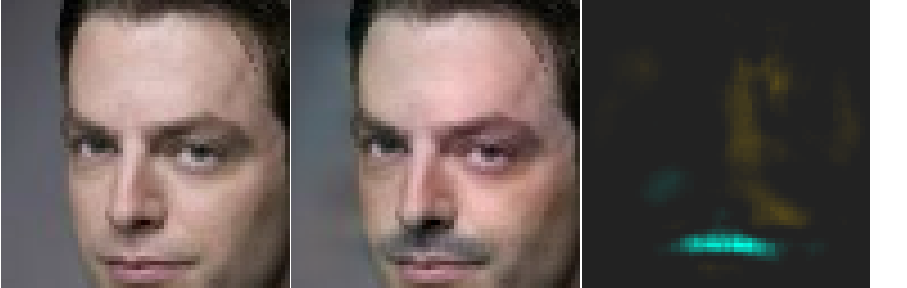
\includegraphics[width=1\linewidth]{img/fooling/AddingMoustache_35_HKR.png}
%      \label{fig:AddingMoustache_1_OK}
%    \end{subfigure}%
%    \begin{subfigure}{.25\textwidth}
%      \centering
%      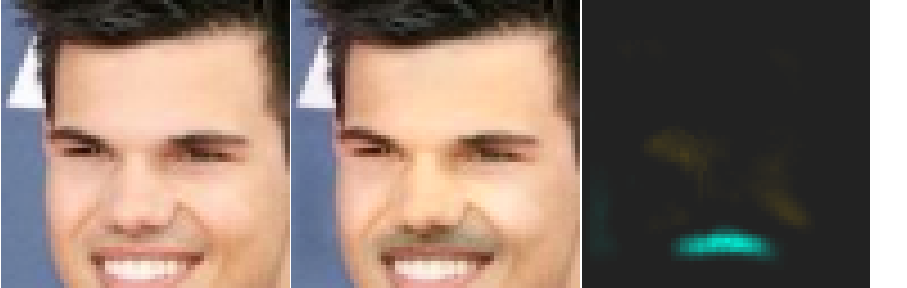
\includegraphics[width=1\linewidth]{img/fooling/AddingMoustache_58_HKR.png}
%      \label{fig:AddingMoustache_5_OK}
%    \end{subfigure}
%    \begin{subfigure}{.25\textwidth}
%      \centering
%      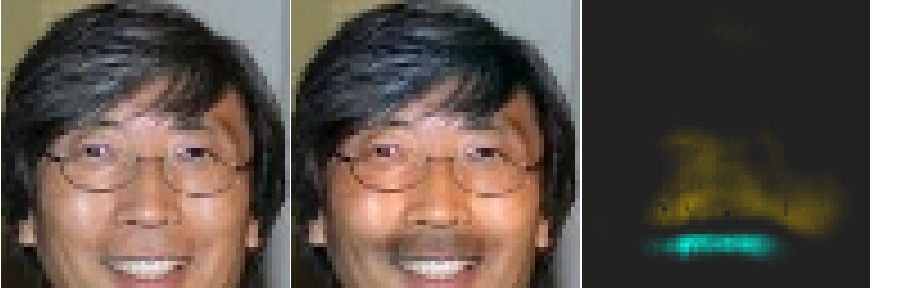
\includegraphics[width=1\linewidth]{img/fooling/AddingMoustache_54_HKR.png}
%      \label{fig:AddingMoustache_3_OK}
%    \end{subfigure}%
%    \begin{subfigure}{.25\textwidth}
%      \centering
%      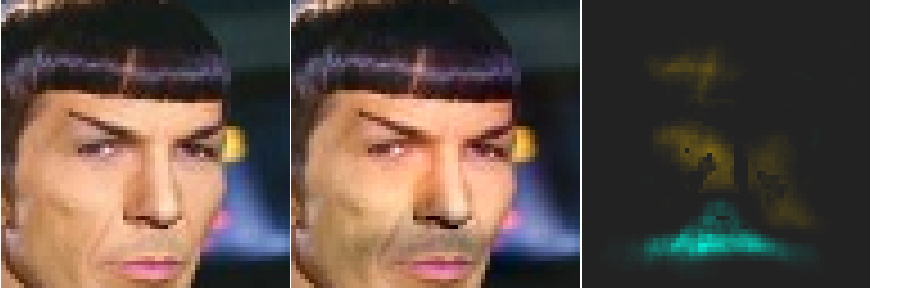
\includegraphics[width=1\linewidth]{img/fooling/AddingMoustache_218_HKR.png}
%      \label{fig:AddingMoustache_4_OK}
%    \end{subfigure}
%    \caption{Fooling "non-moustache" images with the proposed Hinge-KR classifier}
%\end{subfigure}  
%\begin{subfigure}{1.\textwidth}
%    \begin{subfigure}{.25\textwidth}
%      \centering
%      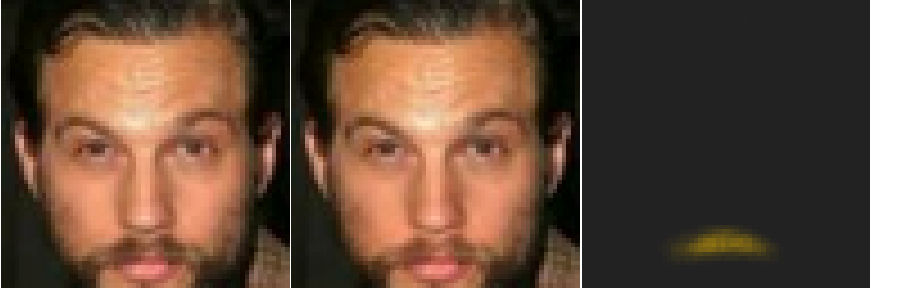
\includegraphics[width=1\linewidth]{img/fooling/remove_mustache_6008.png}
%      \label{fig:RemovingMoustache_4_OK}
%    \end{subfigure}%
%    \begin{subfigure}{.25\textwidth}
%      \centering
%      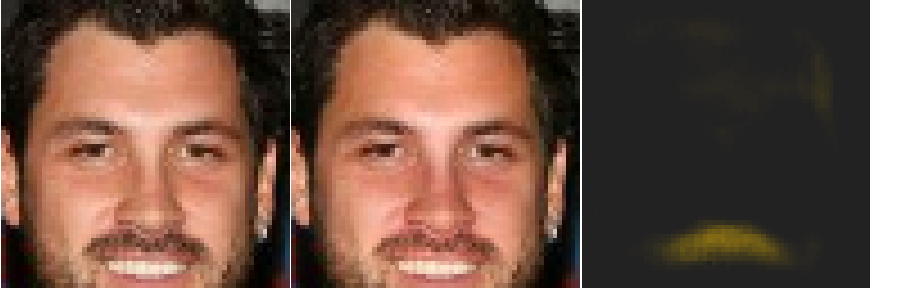
\includegraphics[width=1\linewidth]{img/fooling/remove_mustache_1489.png}
%      \label{fig:RemovingMoustache_2_OK}
%    \end{subfigure}
%    \begin{subfigure}{.25\textwidth}
%      \centering
%      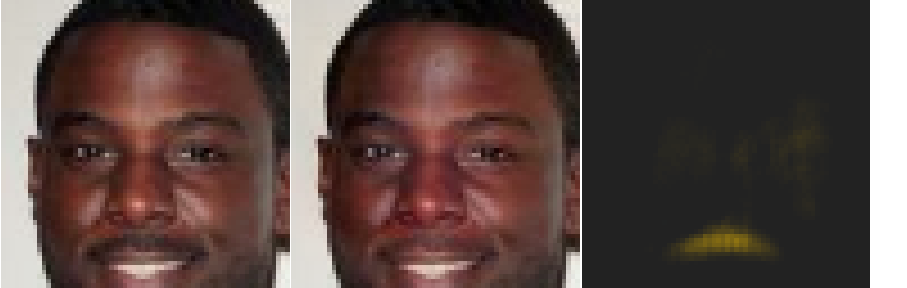
\includegraphics[width=1\linewidth]{img/fooling/remove_mustache_6850.png}
%      \label{fig:RemovingMoustache_5_OK}
%    \end{subfigure}%
%    \begin{subfigure}{.25\textwidth}
%      \centering
%      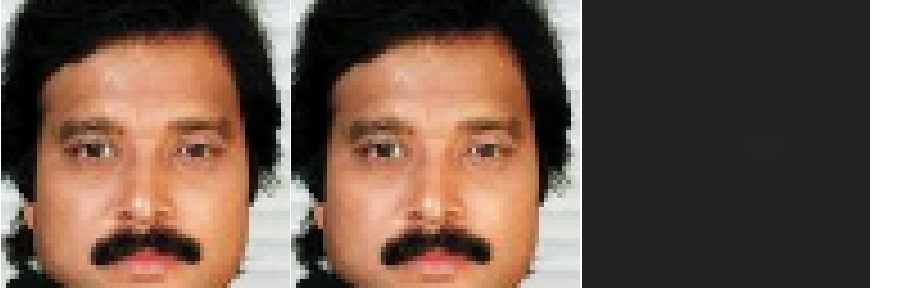
\includegraphics[width=1\linewidth]{img/fooling/remove_mustache_1604.png}
%      \label{fig:RemovingMoustache_1_KO}
%    \end{subfigure}
%\caption{Fooling "moustache" images with the proposed Hinge-KR classifier}
%\end{subfigure}  
%\caption{Deepfool adversarial examples  on Celeb-A dataset. Classical networks and 1-lipschitz networks learned with binary crossentropy lead to invisble noise, whereas proposed solution add or remove dark pixels around the nasolabial fold}
%\label{fig:Deep_fool_CelebA}
%\end{figure}

\begin{figure}
\centering
\begin{subfigure}{1.\textwidth}
    \begin{subfigure}{.245\textwidth}
      \centering
      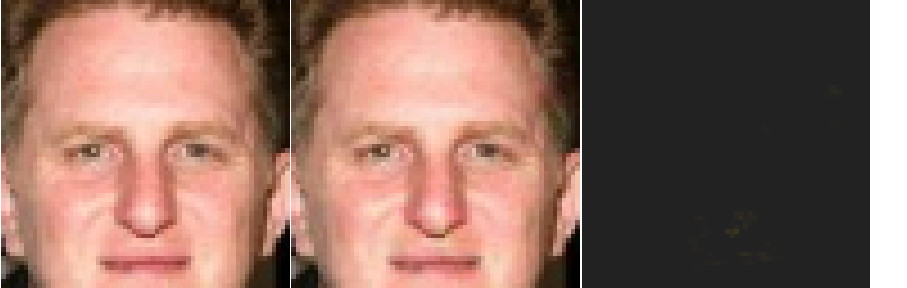
\includegraphics[width=1\linewidth]{img/fooling/AddingMoustache_52_Classic.png}
      \label{fig:AddingMoustache_52_Classical}
    \end{subfigure}%
    \begin{subfigure}{.245\textwidth}
      \centering
      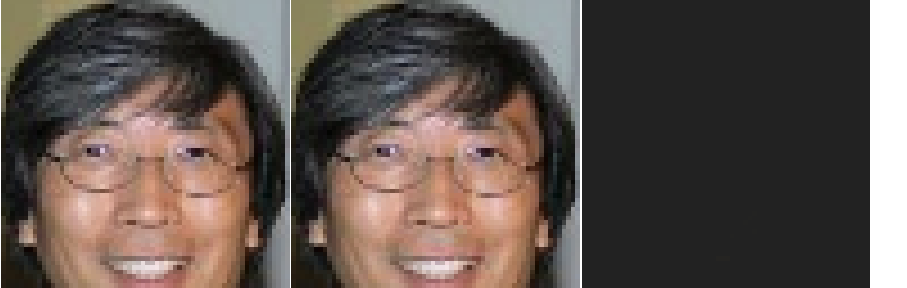
\includegraphics[width=1\linewidth]{img/fooling/AddingMoustache_54_Classic.png}
      \label{fig:AddingMoustache_54_Classical}
    \end{subfigure}  
    \begin{subfigure}{.245\textwidth}
      \centering
      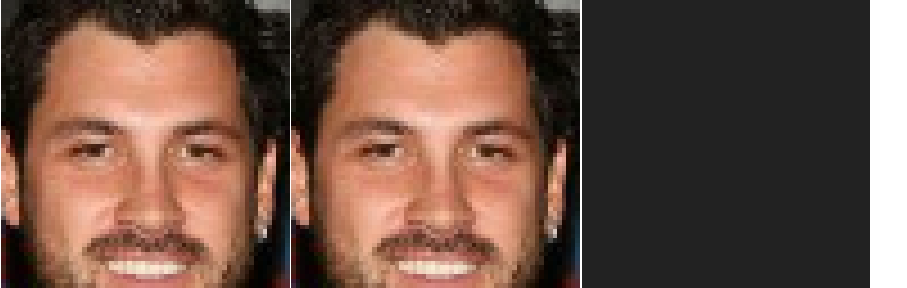
\includegraphics[width=1\linewidth]{img/fooling/remove_mustache_1489_Classic.png}
      \label{fig:remove_mustache_1489}
    \end{subfigure}  
    \begin{subfigure}{.245\textwidth}
      \centering
      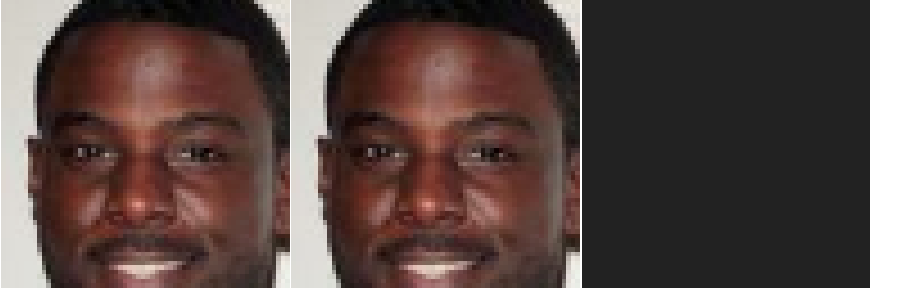
\includegraphics[width=1\linewidth]{img/fooling/remove_mustache_6850_Classic.png}
      \label{fig:remove_mustache_6850}
    \end{subfigure}  
    \caption{Fooling CelebA images classical network}
\end{subfigure}  

\begin{subfigure}{1.\textwidth}
    \begin{subfigure}{.245\textwidth}
      \centering
      \includegraphics[width=1\linewidth]{img/fooling/AddingMoustache_52_1LipSigmoid.png}
      \label{fig:AddingMoustache_52_Lip_binCross}
    \end{subfigure}%
    \begin{subfigure}{.245\textwidth}
      \centering
      \includegraphics[width=1\linewidth]{img/fooling/AddingMoustache_54_1LipSigmoid.png}
      \label{fig:AddingMoustache_54_Lip_binCross}
    \end{subfigure} 
    \begin{subfigure}{.245\textwidth}
      \centering
      \includegraphics[width=1\linewidth]{img/fooling/remove_mustache_1489_1LipSigmoid.png}
      \label{fig:remove_mustache_1489_Lip_binCross}
    \end{subfigure}  
    \begin{subfigure}{.245\textwidth}
      \centering
      \includegraphics[width=1\linewidth]{img/fooling/remove_mustache_6850_1LipSigmoid.png}
      \label{fig:remove_mustache_6850_Classic}
    \end{subfigure}  
    \caption{Fooling images 1-lipschitz network (binary crossentropy)}
\end{subfigure}  
\begin{subfigure}{1.\textwidth}
    \begin{subfigure}{.245\textwidth}
      \centering
      \includegraphics[width=1\linewidth]{img/fooling/AddingMoustache_52_HKR.png}
      \label{fig:AddingMoustache_1_OK}
    \end{subfigure}%
    \begin{subfigure}{.245\textwidth}
      \centering
      \includegraphics[width=1\linewidth]{img/fooling/AddingMoustache_54_HKR.png}
      \label{fig:AddingMoustache_5_OK}
    \end{subfigure}
    \begin{subfigure}{.245\textwidth}
      \centering
      \includegraphics[width=1\linewidth]{img/fooling/remove_mustache_1489_hKR.png}
      \label{fig:AddingMoustache_3_OK}
    \end{subfigure}%
    \begin{subfigure}{.245\textwidth}
      \centering
      \includegraphics[width=1\linewidth]{img/fooling/remove_mustache_6850_hKR.png}
      \label{fig:AddingMoustache_4_OK}
    \end{subfigure}
    \caption{Fooling images with the proposed hinge-KR classifier}
\end{subfigure}  
\begin{subfigure}{1.\textwidth}
    \begin{subfigure}{.245\textwidth}
      \centering
      \includegraphics[width=1\linewidth]{img/adding_mustache_52_k2.png}
      \label{fig:AddingMoustache_grad_1_OK}
    \end{subfigure}%
    \begin{subfigure}{.245\textwidth}
      \centering
      \includegraphics[width=1\linewidth]{img/adding_mustache_54_k4.png}
      \label{fig:AddingMoustache_grad_5_OK}
    \end{subfigure}
    \begin{subfigure}{.245\textwidth}
      \centering
      \includegraphics[width=1\linewidth]{img/remove_mustache_1489_k10.png}
      \label{fig:AddingMoustache_grad_3_OK}
    \end{subfigure}%
    \begin{subfigure}{.245\textwidth}
      \centering
      \includegraphics[width=1\linewidth]{img/remove_mustache_6950_k10.png}
      \label{fig:AddingMoustache_grad_4_OK}
    \end{subfigure}
    \caption{Counterfactuals for hinge-KR classifier using gradient with resp. $c_x=2,4,10,10$}
\end{subfigure}
\caption{(a-c) Deepfool and adversarial examples  on Celeb-A dataset: two left (resp. right) triplet-images without (resp. with) mustache. Triplet-images consist of source image, fooled image, and differential image of V channel in HSV colorspace (yellow (resp. cyan) increase (resp. decrease) V channel level) with a common color scale for all settings. (d) counterfactuals: the last images of the triplets are $\nabla_x \hat{f}(\textbf{x})$ with the same color representation than differential images.}
%Classical networks (1st line) and 1-lipschitz networks learned with binary crossentropy (2nd line) lead to invisble noise, whereas proposed solution (3rd line) add or remove dark pixels around the nasolabial fold}
\label{fig:Deep_fool_CelebA}
\end{figure}

% \begin{figure}{1.\textwidth}
%     \begin{subfigure}{.245\textwidth}
%       \centering
%       \includegraphics[width=1\linewidth]{img/adding_mustache_52_k2.png}
%       \label{fig:AddingMoustache_1_OK}
%     \end{subfigure}%
%     \begin{subfigure}{.245\textwidth}
%       \centering
%       \includegraphics[width=1\linewidth]{img/adding_mustache_54_k4.png}
%       \label{fig:AddingMoustache_5_OK}
%     \end{subfigure}
%     \begin{subfigure}{.245\textwidth}
%       \centering
%       \includegraphics[width=1\linewidth]{img/remove_mustache_1489_k9.png}
%       \label{fig:AddingMoustache_3_OK}
%     \end{subfigure}%
%     \begin{subfigure}{.245\textwidth}
%       \centering
%       \includegraphics[width=1\linewidth]{img/remove_mustache_6950_k10.png}
%       \label{fig:AddingMoustache_4_OK}
%     \end{subfigure}
%     \caption{Counterfactuals for hinge-KR classifier using gradient with resp. $c_x=2,4,9,10$}
% \end{figure}

 
%We claim that the output of the proposed method can be used as a confidence criteria in the decision..... %\footnote{{\color{red} TBC }}


\section{Conclusion and future works}
This paper presents a novel binary classification framework and the associated deep learning process. Besides the interpretation of the classification task as a regularized optimal transport problem, we demonstrate that this new formalization has some valuable properties about error bounds and robustness regarding adversarial attacks. We also propose a systematic approach to ensure the 1-Lipschitz constraint of a neural network. This includes a state-of-the-art regularization algorithm and more precise constant evaluation for convolutional and pooling layers. Even if this regularization process can increase the computation time during learning, it doesn't impact inference. We developed an open source python library based on tensorflow for 1-Lipshitz layers and gradient preserving activation and pooling functions. This makes the approach very easy to implement and to use. \\

The experiment emphasizes the theoretical results and confirms that the classifier has good and predictable robustness to adversarial attack with a acceptable cost on accuracy. We also show that our classifier forces adversarial attacks to explicitly modify the input. Moreover, we show that we can easily build counterfactuals explanations. This suggest that with our novel classification problem, the adversarial attack is linked to the optimal transportation.

In conclusion, we believe that this classification framework based on optimal transport is of great interest for critical problems since it provides both empirical and theoretical guarantees. Future works will focus on the multiclass counterpart of the approach and on its applicability to large and deep networks.

%\if@submission \@submission false
\acksection
This project received funding from the French ”Investing for the Future – PIA3” program within the Artificial and Natural Intelligence Toulouse Institute (ANITI). The authors gratefully acknowledge the support of the DEEL project\footnote{https://www.deel.ai/}.
%\fi
\if@submission \@submission true
\newpage
\section*{Broader Impact}
Machine learning, and more precisely deep learning, is one of the rare areas of science where the adoption by the industry drives the research.  Major empirical and theoretical progress in deep learning raise unprecedented enthusiasm.  Thus, machine learning is used in more and more applications that can have a major impact on humanity such as medical and juridical applications, autonomous transportation and so on.  However, deep learning approach suffers from two major flaws in this context:  a lack of theoretical guarantee (error bounds, convergence rate…) and a structural weakness to adversarial attacks. The author’s team research areas are the certification of machine algorithms, the robustness and the explainability of neural networks. 
We believe that the current paper may have a significant impact on both the theoretical machine learning and industrial applications. On the theoretical side, we propose a novel classification framework that establish the link between machine learning and optimal transport. We provide theoretical guarantees of existence and optimality in terms of classification.  It gives an interpretation of classification and adversarial attack in terms of optimal transport. The proposed loss function enables a tradeoff between robustness and accuracy. We prove that the output of our classifier is always a lower bound (which can be very tight) of the robustness with respect to adversarial attacks. This means that any prediction of the model comes with an interpretable robustness level.  All of these guarantees may help a lot to certify this type of approach.

On the practical side, the framework requires strong constraint on neural networks. This led us to use quite uncommon neural networks layers with sorting activation functions, norm preserving pooling and orthonormalized weights. With this architecture, the theoretical requirements are fulfilled and then, the robustness lower bounds are guaranteed in practice. To make this approach accessible to researchers and industry, we propose an open source library based on Tensorflow. 

Last, we empirically show that our approach is robust to adversarial attacks and that adversarial attacks explicitly build counterfactual examples. We also show that the gradient of the network's output can be used to easily obtain such counterfactuals .  This provides a simple method to explain the predictions of models learned with our framework.
% pas sûr de la formulation: The downsides are twice

The approach has two limitations. First, the energy footprint of the learning process in our approach is between two and three times larger than classical ones (however, the difference becomes negligible in inference). The second is the small decrease in terms of accuracy.

In conclusion, we show that our method provides both theoretical and structural guarantees. The predictions are interpretable and associated with a robustness lower bound. We strongly believe that this kind of approach may help to guarantee the safety of deep learning algorithms, especially for critical tasks.
\newpage
\fi
\bibliographystyle{plain}
\bibliography{biblio} 



\newpage
\appendix
%\begin{center}

% {\huge \textbf{Appendix \\ Achieving robustness in classification using optimal transport with hinge regularization}}
% \end{center}
\section{Optimal transportation : discrete case}
\subsection{Optimal transport}
\label{secOptTransp}
When considering a limited number of samples for the two distribution, the computation of the Wasserstein distance 
%is an optimal transportation problem that 
can be solved through linear programming algorithms. In the balanced case, we have $X=\{x_1, \ldots, x_{2n}\}$ where $\{x_1,\ldots,x_n\}$ are sampled from $P_+$ and  $\{x_{n+1},\ldots,x_{2n}\}$ are sampled from $P_-$. We note $U=\{u_1, \ldots, u_{2n}\}$ the labels with $u_1,\ldots,u_n=1$ and $u_{n+1},\ldots,u_{2n}=-1$ and $C$ the $n\times n$ matrix cost function with $C_{i,j}=||x_i-x_{n+j}||$. The primal problem of the optimal transport is to find a transportation plan $\Pi$ (a $n\times n$ matrix) such as:
\begin{alignat}{2}
&\!\min_{\Pi}        &\qquad& \sum_{i,j \in n\times n}\Pi_{i,j}*C_{i,j}\\
&\text{subject to} &      & \Pi_{i,j} \geq 0,\\
&                  &      & \sum_i \Pi_{i,j} = \frac{1}{n},\sum_j \Pi_{i,j} = \frac{1}{n}.
\end{alignat}
The constraints enforce $\Pi$ to be a discrete joint probability distribution with the appropriate marginals as in the continuous case. The dual formulation for the discrete optimal transport problem is:
\begin{alignat}{2}
&\!\max_{F}        &\qquad& F.U^T\\
&\text{subject to} &      & \forall i,j \in n\times n, F_i-F_{n+j}\leq C_{i,j}
\end{alignat}
where $F$ is a $2n$ vector that is a discrete version of the function $f$ of Equation \ref{kantorovich}. The constraint on $F$ is the discrete counterpart of the 1-Lipschitz constraint. 

\subsection{Hinge regularized Optimal transport}
Similarly to the classical case, the discrete counterpart of the regularized Wasserstein distance is also a transportation problem which has the following formulation:
\begin{alignat*}{2}
&\!\min_{\Pi}        &\qquad& \sum_{i,j \in n\times n}\left[\Pi_{i,j}*C_{i,j}\right]-2\left(1-\sum_{i,j \in  n\times n}\left[\Pi_{i,j}\right]\right)\\
&\text{subject to} &      & \Pi_{i,j} \geq 0,\\
&                  &      & \frac{1}{n} \leq \sum_i \Pi_{i,j} \leq  \frac{1+\lambda}{n},\\
&                  &      & \frac{1}{n} \leq \sum_j \Pi_{i,j} \leq  \frac{1+\lambda}{n}.
\end{alignat*}
Roughly speaking, it allows to give more weight to the transportation of the closest pairs by admitting to deviate from the marginals with a tolerance that depends on $\lambda$. Since the closest pairs in the two distributions are the most difficult to classify, it illustrates why this formulation is more adequate for classification problem. 
The dual formulation of this transportation problem is a discrete counterpart of Equation \ref{eq:reg_OT} :
\begin{alignat*}{2}
&\!\max_{F}        &\qquad& \sum_{k =0}^{2n} \left[F_i*u_i -\lambda (0,1-F_i*u_i)_+\right]\\
&\text{subject to} &      & \forall i,j \in n\times n, F_i-F_{n+j}\leq C_{i,j}.
\end{alignat*}
We observe that the constraint in the dual problem are not affected by the new formulation and still corresponds to a the 1-Lipschitz constraint in the continuous case. 


\section{Theorem proofs}
\label{appendix:proofs}
\subsection{Proof Theorem 1}
We denote as 
\begin{align}\label{eq:defwoth}
	f^*:=f_{\lambda}^*\in{\arg\min}_{f\in \text{Lip}_1(\Omega)}\mathcal{L}^{hKR}_\lambda(f)\ \ \text{and} \ \ \hat{f}_n:=\hat{f}_{n,\lambda}\in{\arg\min}_{f\in \text{Lip}_1(\Omega)}\hat{\mathcal{L}}^{hKR}_{\lambda,n}(f).
\end{align}
If we assume that \eqref{eq:M} is not true, then there exists $\textbf{x}\in \Omega$ such that $f^*(\textbf{x})>1+\text{diam}(\Omega)+\frac{\mathcal{R}(\psi)}{\inf(p,1-p)}$ or $f^*(\textbf{x})<-1-\text{diam}(\Omega)-\frac{L_1(\psi)}{\inf(p,1-p)}$. We suppose without loss of generality that the first inequality holds. If ${{\textbf{z}}}\in \Omega $ then the 1-Lipschitz condition in $f^*$ implies that $f^*({{\textbf{z}}})>1+\frac{L_1(\psi)}{1-p}$. Hence $(1-f^*)_+=0$ and
\begin{align*}
	L(f^*)&\leq \sup_{g\in Lip_1(\Omega)} L_2(g)- \lambda L_1(f^*)\\
	&=\sup_{g\in Lip_1(\Omega)}E_{X|Y=1}(g(X))-E_{X|Y=-1}(g(X))-E\left\{\lambda (1-Yf^*(X))_+\right\}\\
	&= L_2(\psi)-\lambda \{ pE_{X|Y=1}(1-f^*(X))_++(1-p)E_{X|Y=-1}(1+f^*(X))_+\}\\
	&\leq L_2(\psi)-\lambda \{ (1-p)E_{X|Y=-1}(1+f^*(X))\}\\
	&\leq  L_2(\psi)-\lambda \{ (1-p)E_{X|Y=-1}(2+\frac{L_1(\psi)}{1-p})\} \\
	&= L_2(\psi)-2\lambda(1-p) -\lambda \{ E_{X|Y=-1}({L_1(\psi)})\}=L_2(\psi)-2\lambda(1-p)-\lambda L_1(\psi) 
\end{align*}
Then $f^*$ can not be an optimal solution of the problem \eqref{eq:defwoth}. Then there exists some constant $M$ large enough, such that $f^*$ belongs to $\text{Lip}^M_1(\Omega):=\{f\in \text{Lip}_1(\Omega): || f||_{\infty}\leq M\}$ and not to $\text{Lip}_1(\Omega)$. Since the functional $\mathcal{L}^{hKR}_\lambda$ is convex and $\text{Lip}^M_1(\Omega)$ is compact in $\mathcal{C}(\Omega)$, we are able to make use of Ascoli-Arzela Theorem and conclude that there exists at least one function minimizing the expected loss. Furthermore the set of those functions is compact and convex.


\subsection{Proof Theorem 2}
\begin{Definition}
Let $\mu, \nu$ two positive measures in $\R^d$. The Kullback-Leibler divergence from $\mu$ to $\nu$ is defined as 
\begin{align}
KL(\mu |\nu )=\begin{cases} 
      \int \log(\frac{d\mu}{d\nu})d\mu-\int d\mu+\int d\nu & \text{if} \ \ \mu  << \nu\\
      \infty & otherwise 
   \end{cases}
\end{align}
\end{Definition}
\begin{Theorem}\label{Theo:generaldual}
Let $\phi_1, \phi_2:\Omega\rightarrow \bar{\R}$ be lower semicontinuous convex functions and $\mu, \nu\in \mathcal{P}(\Omega)$ be probability measures. Then for all $\epsilon>0$ the following equality holds
\begin{align}\label{eq:dual_app}
\begin{split}
	&\inf_{\pi \in\Pi_+(\mu, \nu)} \int{\phi_1(-\frac{d\pi_\textbf{x}}{d\mu}(\textbf{x}))d\mu}(\textbf{x})+\int{\phi_2(-\frac{d\pi_{{\textbf{z}}}}{d\nu}({{\textbf{z}}}))d\nu}({{\textbf{z}}})+\epsilon KL(\pi|e^{-\frac{c(\textbf{x},{{\textbf{z}}})}{\epsilon}}(d\mu\times d\nu))\\&= \sup_{f,g\in L^1(\Omega)}-\int_{\Omega}\phi_1^*(f(\textbf{x}))d\mu(\textbf{x})-\int_{\Omega}\phi_1^*(g({{\textbf{z}}}))d\nu({{\textbf{z}}})-\epsilon \int \left(e^{\frac{f(\textbf{x})+g({{\textbf{z}}})-c(\textbf{x},{{\textbf{z}}})}{\epsilon}}-e^{-\frac{c(\textbf{x},{{\textbf{z}}})}{\epsilon}}\right)d\mu d\nu.
	\end{split}
\end{align}
Furthermore if $\epsilon=0$ then
\begin{align}\label{eq:dual_app_zero}
\begin{split}
	&\inf_{\pi \in\Pi_+(\mu, \nu)}\int_{\Omega\times \Omega}c(\textbf{x},{{\textbf{z}}})d\pi(\textbf{x},{{\textbf{z}}}) + \int{\phi_1(-\frac{d\pi_\textbf{x}}{d\mu}(\textbf{x}))d\mu}(\textbf{x})+\int{\phi_2(-\frac{d\pi_{{\textbf{z}}}}{d\nu}({{\textbf{z}}}))d\nu}({{\textbf{z}}})\\&= \sup_{(f,g)\in \Phi(\mu, \nu)}-\int_{\Omega}\phi_1^*(f(\textbf{x}))d\mu(\textbf{x})-\int_{\Omega}\phi_1^*(g({{\textbf{z}}}))d\nu({{\textbf{z}}}).
	\end{split}
\end{align}
Where $\Pi_+(\mu, \nu)$ is the set of positive measures $\pi\in \mathcal{M}_+(\Omega\times \Omega)$ which are absolutely continuous  with respect to the joint measure $d\mu\times d\nu$, and $\Phi(\mu, \nu)$ consists of the pairs of functions $(f,g)\in L_1(\Omega)\times L_1(\Omega)$ such that $c(\textbf{x},{{\textbf{z}}})-f(\textbf{x})-g({{\textbf{z}}}) \geq 0$ $ d\mu\times d\nu -a.s.$.
\end{Theorem}

First we recall the Fenchel–Rockafellar Duality result, we use a weaker version given in Theorem 1.12 in \cite{Brez}
\begin{Proposition} \label{Fenchel–Rockafellar}
Let $E$ be a Banach space and $\Upsilon,\Psi:E\rightarrow \R \cup \{\infty \}$ be two convex functions, assume that there exist ${{\textbf{z}}}_0\in\text{dom}(\Psi)\cap \text{dom}(\Upsilon) $ such that $\Psi$ is continous in ${{\textbf{z}}}_0$. Then strong duality holds
\begin{align} \label{FC}
\inf_{a\in E}\left\lbrace \Upsilon(a)+\Psi(a)\right\rbrace=\sup_{b\in E^*}\left\lbrace -\Upsilon^*(-b)-\Psi^*(b)\right\rbrace
\end{align}
\end{Proposition} 
We identify the different elements of our problem with such of previous Proposition. 
\begin{itemize}
\item $E$ is the space of continuous functions in $\Omega\times \Omega$. Note that the set is bounded, hence $E^*$, by Riesz theorem, is the set of regular measures in $\Omega\times \Omega$.
\item If $\epsilon=0:$
\begin{align}
\Psi_0(u)&=\begin{cases} 
      0 & \text{if} \ \ u(\textbf{x},{{\textbf{z}}})\geq -c(\textbf{x},{\textbf{z}})\\
      \infty & \text{otherwise }
   \end{cases}\\ 
\Upsilon_0(u)&= \begin{cases} 
      \int \phi_1^*(-f(\textbf{x}))d\mu(\textbf{x})+\int \phi_2^*(-g({{\textbf{z}}})) d\nu({{\textbf{z}}})  & \text{if} \ \ u(\textbf{x},{\textbf{z}})=f(\textbf{x})+g({\textbf{z}})\\ 
      \infty & \text{otherwise } 
   \end{cases}
\end{align}
If $\epsilon>0$:
\begin{align}
\Psi_{\epsilon}(u)&=\epsilon \int \left(e^{\frac{u(\textbf{x},{{\textbf{z}}})-c(\textbf{x},{\textbf{z}})}{\epsilon}}-e^{-\frac{c(\textbf{x},{\textbf{z}})}{\epsilon}}\right)d\mu(\textbf{x}) d\nu({{\textbf{z}}})\\ 
 \Upsilon_{\epsilon}(u)&=\Upsilon_0(u)
\end{align}
\end{itemize}
Note that $ \Upsilon_{\epsilon}(u)=\Upsilon_0(u)$ could be non well defined, to avoid this situation we fix $\textbf{x}_0\in \Omega$ and consider $u(\textbf{x},{{\textbf{z}}})=(u(\textbf{x},{{\textbf{z}}}_0)-u({{\textbf{z}}}_0,{{\textbf{z}}}_0)/2)+u({{\textbf{z}}}_0,{{\textbf{z}}})-u({{\textbf{z}}}_0,{{\textbf{z}}}_0)/2)$. 
Now we compute the dual operators 
\begin{align*}
\Psi^*_{\epsilon}(-\pi)&=\sup_{u\in E}\left\lbrace  -\epsilon\int \left(e^{\frac{u(\textbf{x},{{\textbf{z}}})-c(\textbf{x},{\textbf{z}})}{\epsilon}}-e^{-\frac{c(\textbf{x},{\textbf{z}})}{\epsilon}}\right)d\mu(\textbf{x}) d\nu({{\textbf{z}}})-\int u(\textbf{x},{\textbf{z}})d\pi(\textbf{x},{{\textbf{z}}}) \right\rbrace\\
&=\sup_{u\in E}\left\lbrace -\epsilon\int \left(e^{\frac{u(\textbf{x},{\textbf{z}})-c(\textbf{x},{{\textbf{z}}})}{\epsilon}}-e^{-\frac{c(\textbf{x},{{\textbf{z}}})}{\epsilon}}\right)d\mu(\textbf{x}) d\nu({{\textbf{z}}})+\int u(\textbf{x},{{\textbf{z}}})d\pi(\textbf{x},{{\textbf{z}}}) \right\rbrace
\end{align*}
Now if $\pi$ were not absolutely continuous respect the joint measure $e^{-\frac{c(\textbf{x},{{\textbf{z}}})}{\epsilon}}d\mu\times d\nu$ then we would have a continuous function $u(\textbf{x},{{\textbf{z}}})=0$ $d\mu\times d\nu$ almost surely and such that $\int u(\textbf{x},{{\textbf{z}}})d\pi(\textbf{x},{{\textbf{z}}})\neq 0$. If we take the function $\lambda u({{\textbf{z}}},{{\textbf{z}}})$ and $\lambda$ tends to $\pm \infty$ we deduce that the supremum is $\infty $. Then suppose that $d\pi =m(\textbf{x},{{\textbf{z}}})e^{-\frac{c(\textbf{x},{{\textbf{z}}})}{\epsilon}}(d\mu\times d\nu)$.
\begin{align*}
\Psi^*_{\epsilon}(-\pi)&= \begin{cases} 
      \sup_{u\in E}\left\lbrace \epsilon\int \left(-e^{\frac{u(\textbf{x},{{\textbf{z}}})}{\epsilon}}+1 +\frac{u(\textbf{x},{{\textbf{z}}})}{\epsilon}m(\textbf{x},{{\textbf{z}}})\right) e^{-\frac{c(\textbf{x},{{\textbf{z}}})}{\epsilon}}d\mu(\textbf{x}) d\nu({{\textbf{z}}}) \right\rbrace & \text{if $d\pi =m e^{-\frac{c(\textbf{x},{{\textbf{z}}})}{\epsilon}}(d\mu\times d\nu)$.} \\
      \infty & \text{otherwise. } 
   \end{cases}\\
   &=  \epsilon KL(\pi|e^{-\frac{c(\textbf{x},{{\textbf{z}}})}{\epsilon}}(d\mu\times d\nu) ) & 
\end{align*}
With some similar calculation, we compute for $\epsilon=0$:
\begin{align*}
\Psi^*_{0}(-\pi)&= \begin{cases} 
     \int c(\textbf{x},{{\textbf{z}}})d\pi(\textbf{x},{{\textbf{z}}}) & \text{if $\pi$ is a positive measure.} \\
      \infty & \text{otherwise. } 
   \end{cases}
\end{align*}
Finally for $\Upsilon^*_{\epsilon}=\Upsilon^*_{0}$
\begin{align*}
\Upsilon^*_{\epsilon}(\pi)&=\sup_{u\in E,\  u(\textbf{x},{{\textbf{z}}})=f(\textbf{x})+g({{\textbf{z}}}) }\left\lbrace \int f(\textbf{x})+g({{\textbf{z}}}) d\pi(\textbf{x},{{\textbf{z}}})-\int \phi_1^*(-f(\textbf{x}))d\mu(\textbf{x}) -\int \phi_2^*(-g({{\textbf{z}}})) d\nu({{\textbf{z}}})\right\rbrace\\
 &=\sup_{u\in E,\  u(\textbf{x},{{\textbf{z}}})=f(\textbf{x})+g({{\textbf{z}}}) }\left\lbrace \int f(\textbf{x})d\pi_\textbf{x}(\textbf{x})-\int \phi_1^*(-f(\textbf{x}))d\mu(\textbf{x}) +\int g({{\textbf{z}}}) d\pi_{{\textbf{z}}}({{\textbf{z}}})-\int \phi_2^*(-g({{\textbf{z}}})) d\nu({{\textbf{z}}})\right\rbrace\\
  &=\sup_{f \in C(\Omega)}\left\lbrace \int f(\textbf{x})d\pi_\textbf{x}(\textbf{x})-\int \phi_1^*(-f(\textbf{x}))d\mu(\textbf{x})\right\rbrace +\sup_{g\in C(\Omega) }\left\lbrace \int g({{\textbf{z}}}) d\pi_{{\textbf{z}}}({{\textbf{z}}})-\int \phi_2^*(-g({{\textbf{z}}})) d\nu({{\textbf{z}}})\right\rbrace\\
  &=(I_1)+(I_2).
\end{align*}
We first consider  $(I_1)$. The same reasoning will hold for $(I_2)$. If $\pi_\textbf{x}$ were not absolutely continuous respect $\mu$ then reasoning as before we obtain $\infty$. Then $d \pi_\textbf{x}=\frac{d\pi_\textbf{x}}{d\mu}d\mu$ and
\begin{align*}
(I_1)&=\sup_{f \in C(\Omega)}\left\lbrace \int \left( -f(\textbf{x})\frac{d\pi_\textbf{x}}{d\mu}-\phi_1^*(f(\textbf{x})))\right)d\mu(\textbf{x})\right\rbrace\\
&=\int \left( \sup_{m}\left\lbrace -\frac{d\pi_\textbf{x}}{d\mu}m- \phi_1^*(m))\right\rbrace\right)d\mu(\textbf{x})=\int \phi_1(-\frac{d\pi_\textbf{x}}{d\mu})d\mu(\textbf{x})\\
(I_2)&=\int \phi_2(-\frac{d\pi_\textbf{x}}{d\nu})d\mu({{\textbf{z}}})
\end{align*}
Note that the inversion of the  supremum and  the integral  is guaranteed here since $(\textbf{x},m)\mapsto -m\frac{d\pi_\textbf{x}}{d\mu}(\textbf{x})+\phi_1^*(m)$ is lower semi-continuous and convex in $m$ and measurable in $(\textbf{x},m)$. Then it is a normal integrand, and we can apply Theorem 14.60 in \cite{RoWe}.\\
Then computing both in Equation \eqref{FC} we end with the following result
\begin{align*}
\inf_{ u(\textbf{x},{\textbf{{{\textbf{z}}}}})=f(\textbf{x})+g({\textbf{{{\textbf{z}}}}})\geq -c(\textbf{x},{{\textbf{z}}})}&\left\lbrace \int \phi_1^*(-f(\textbf{x}))d\mu(\textbf{x})+\int \phi_2^*(-g({{\textbf{z}}})) d\nu({{\textbf{z}}})\right\rbrace\\& = \inf_{ f(\textbf{x})+g({{\textbf{z}}})\leq c(\textbf{x},{{\textbf{z}}})}\left\lbrace \int\phi_1^*(f(\textbf{x}))d\mu(\textbf{x})+\int \phi_2^*(g({{\textbf{z}}})) d\nu({{\textbf{z}}})\right\rbrace\\
\\& = -\sup_{ f(\textbf{x})+g({{\textbf{z}}})\leq c(\textbf{x},{{\textbf{z}}})}\left\lbrace -\int \phi_1^*(f(\textbf{x}))d\mu(\textbf{x})-\int \phi_2^*(g({{\textbf{z}}})) d\nu({{\textbf{z}}})\right\rbrace
\end{align*}
\begin{align*}
\sup_{ \pi\in \mathcal{M}_+(\Omega\times \Omega)}&\left\lbrace  -\int c(\textbf{x},{{\textbf{z}}})d\pi(\textbf{x},{\textbf{{{\textbf{z}}}}})-\int \phi_2(-\frac{d\pi_\textbf{x}}{d\nu})d\mu({{\textbf{z}}})- \int \phi_1(-\frac{d\pi_\textbf{x}}{d\mu})d\mu(\textbf{x})\right\rbrace\\
=&-\inf_{ \pi\in \mathcal{M}_+(\Omega\times \Omega)}\left\lbrace\epsilon \int c(\textbf{x},{\textbf{{{\textbf{z}}}}})d\pi(\textbf{x},{\textbf{{{\textbf{z}}}}})+\int \phi_2(-\frac{d\pi_\textbf{x}}{d\nu})d\mu({{\textbf{z}}})+ \int \phi_1(-\frac{d\pi_\textbf{x}}{d\mu})d\mu(\textbf{x})\right\rbrace.
\end{align*}
\begin{align*}
\inf_{ u(\textbf{x},{\textbf{{{\textbf{z}}}}})=f(\textbf{x})+g({\textbf{{{\textbf{z}}}}})}&\left\lbrace \epsilon \int \left(e^{\frac{-f(\textbf{x})-g({\textbf{{{\textbf{z}}}}})-c(\textbf{x},{\textbf{{{\textbf{z}}}}})}{\epsilon}}-e^{-\frac{c(\textbf{x},{\textbf{{{\textbf{z}}}}})}{\epsilon}}\right)d\mu(\textbf{x}) d\nu({{\textbf{z}}})+\int\phi_1^*(-f(\textbf{x}))d\mu(\textbf{x})+\int \phi_2^*(-g({{\textbf{z}}})) d\nu({{\textbf{z}}})\right\rbrace\\ & = \inf_{f,g}\left\lbrace \epsilon \int \left(e^{\frac{f(\textbf{x})+g({\textbf{{{\textbf{z}}}}})-c(\textbf{x},{\textbf{{{\textbf{z}}}}})}{\epsilon}}-e^{-\frac{c(\textbf{x},{\textbf{{{\textbf{z}}}}})}{\epsilon}}\right)d\mu(\textbf{x}) d\nu({{\textbf{z}}})+\int\phi_1^*(f(\textbf{x}))d\mu(\textbf{x})+\int \phi_2^*(g({{\textbf{z}}})) d\nu({{\textbf{z}}})\right\rbrace\\
& = -\sup_{f,g}\left\lbrace -\epsilon \int \left(e^{\frac{f(\textbf{x})+g({\textbf{{{\textbf{z}}}}})-c(\textbf{x},{\textbf{{{\textbf{z}}}}})}{\epsilon}}-e^{-\frac{c(\textbf{x},{\textbf{{{\textbf{z}}}}})}{\epsilon}}\right)d\mu(\textbf{x}) d\nu({{\textbf{z}}})-\int\phi_1^*(f(\textbf{x}))d\mu(\textbf{x})-\int \phi_2^*(g({{\textbf{z}}})) d\nu({{\textbf{z}}})\right\rbrace\\
\end{align*}
\begin{align*}
\sup_{ \pi\in \mathcal{M}_+(\Omega\times \Omega)}&\left\lbrace-\epsilon KL(\pi|e^{-\frac{c(\textbf{x},{\textbf{{{\textbf{z}}}}})}{\epsilon}}(d\mu\times d\nu) )-\int \phi_2(-\frac{d\pi_\textbf{x}}{d\nu})d\mu({{\textbf{z}}})- \int \phi_1(-\frac{d\pi_\textbf{x}}{d\mu})d\mu(\textbf{x})\right\rbrace\\
=&-\inf_{ \pi\in \mathcal{M}_+(\Omega\times \Omega)}\left\lbrace\epsilon KL(\pi|e^{-\frac{c(\textbf{x},{\textbf{{{\textbf{z}}}}})}{\epsilon}}(d\mu\times d\nu) )+\int \phi_2(-\frac{d\pi_\textbf{x}}{d\nu})d\mu({{\textbf{z}}})+ \int \phi_1(-\frac{d\pi_\textbf{x}}{d\mu})d\mu(\textbf{x})\right\rbrace\\
\end{align*}
Proof of Theorem~\ref{Theo:dual}
With the same notation of Theorem \ref{Theo:generaldual}, it is enough to consider, $\mu=P_+$ $\nu=P_-$ and
\begin{align}
	\begin{split}\label{eq:coro:dual_general}
	\psi_1(s)&=\left\{ \begin{array}{lcc}
             p-s &   if  & s\in [p, p+\lambda p]\\
             \\ \infty &  else. &
             \end{array}
   \right.\\
	\end{split}\\
	\begin{split}\label{eq:coro:dual_general2}
	\psi_2(s)&=\left\{ \begin{array}{lcc}
             1-p-s &   if  & s\in [1-p, 1-p+\lambda (1-p)]\\
             \\ \infty &  else. &
             \end{array}
   \right.\\
	\end{split}
\end{align}
 Then for each $f\in L_1(d\mu), \ g\in L_1(d\nu)$
\begin{align*}
-\psi_1^*(f(\textbf{x}))&=-\sup_{s}	\{ -\psi_1(s)+f(\textbf{x})s\}=\inf_{s}	\{ \psi_1(-s)-f(\textbf{x})s\}=\inf_{s}	\{ \psi_1(s)+f(\textbf{x})s\}\\
&=\left\{ \begin{array}{lcc}
             f(\textbf{x}) &   if  & 1\leq f(\textbf{x})\\
             \\ f(\textbf{x})-p\lambda(1-f(\textbf{x})) &  else. &
             \end{array}
   \right.\\&=f(\textbf{x})-p\lambda(1-f(\textbf{x}))_+\\
-\psi_2^*(g(\textbf{{{\textbf{z}}}}))&= f(\textbf{{{\textbf{z}}}})-(1-p)\lambda(1-f(\textbf{{{\textbf{z}}}}))_+.
\end{align*}
Note that when $\lambda\geq 0$ the functions $r\mapsto h_1(r):=r-p\lambda(1-r)_+$ and $h_2(r):=r-(1-p)\lambda(1-r)_+$ are nondecreasing. Now if we denote as $J$ the right hand side of \eqref{eq:dual_app} then 
\begin{align*}
	J=\sup_{(f,g)\in \Phi(\mu, \nu)}\int_{\Omega}h_1(f({\textbf{x}}))d\mu({\textbf{x}})+\int_{\Omega}h_2(g({{\textbf{z}}}))d\mu({{\textbf{z}}}).
\end{align*}
We denote as $f^d$ the $d-$conjugate of $f$ defined as the function
 $$f^d(r):=\inf_{s\in\Omega}{\{ |r-s|-f(s)\}},$$   see for instance in~\cite{GaMc} for a suitable definition. It is clear that $f^{dd}\geq f$, and the equality holds if $f$ is a $d-$concave function since it is said that $f$ is $d-$concave if it is the $d$-conjugate of another function.  Hence using the nondecreasing condition of $h$ we get to
    \begin{align*}
	J=\sup_{f^{dd},f^d}\int_{\Omega}h_1(f^{dd}({\textbf{x}}))d\mu({\textbf{x}})+\int_{\Omega}h_2(f^{d}({{\textbf{z}}}))d\nu({{\textbf{z}}}).
\end{align*}
On the other side $f^d(r)=\inf_{s\in\Omega}{\{ |r-s|-f(s)\}}$ is a limit of a sequence of $1-$Lipschitz functions in $\Omega$, hence it belongs to $\text{Lip}_1(\Omega)$. Using the $1$-Lipschitz property and taking $r=s$ in the infimum leads to 
$$ -f^d(r)\leq  \inf_{s\in\Omega}{\{ |r-s|-f^d(s)\}}\leq -f^d(r).$$ 
This means that $f^{dd}=-f^d(r)$, hence we have that 
\begin{align*}
	J&=\sup_{(-f^d, f^d)}\int_{\Omega}h_1(f^{dd}({\textbf{x}}))d\mu({\textbf{x}})+\int_{\Omega}h_2(f^{d}({{\textbf{z}}}))d\mu({{\textbf{z}}}).\\
	&\leq \sup_{f\in \text{Lip}_1(\Omega)}\int_{\Omega}h_1(f^{dd}({\textbf{x}}))d\mu({\textbf{x}})+\int_{\Omega}h_2(-f({{\textbf{z}}}))d\nu({{\textbf{z}}})\leq J
\end{align*}
where the last inequality comes from the fact that if $f\in\text{Lip}_1(\Omega)$ then $(f,-f)\in \Phi(\mu, \nu)$.

\subsection{Proof Proposition 1}
As a direct consequence of Theorem \ref{Theo:dual} we derive the next equality 
 \begin{align}\label{eq:proofcoro}
\begin{split}
	&\inf_{\pi \in\Pi_{\lambda}(P_+, P_-)}\int_{\Omega\times \Omega}\left(\frac{1}{\epsilon}| {\textbf{x}}-{\textbf{{{\textbf{z}}}}} |-2\right)d\pi  +2\\&= \sup_{f\in \text{Lip}_{1/\epsilon}(\Omega)}\int_{\Omega}f(dP_+-dP_-)-\frac{\lambda}{2} \left( \int_{\Omega}(1-f)_+dP_+ +\int_{\Omega}(1+f)_+dP_-\right).
	\end{split}
\end{align}
We denote as $I$ the left hand side of \eqref{eq:proofcoro} and $\Pi(P_+, P_-)$ the set of measures with marginals $P_+, P_-$. Now using the hypothesis \eqref{coro:hipotesis} we derive the next inequality  
\begin{align*}
	I=\inf_{\pi \in\Pi(P_+, P_-)}\int_{\Omega\times \Omega}\left(\frac{1}{\epsilon}|{\textbf{x}}-{{\textbf{z}}} |-2\right)d\pi+2= \frac{1}{\epsilon}\mathcal{W}(P_+, P_-).
\end{align*}
Since { $\text{Lip}_{1/\epsilon}\mathcal{W}(P_+, P_-)=\sup_{f\in \text{Lip}_{1/\epsilon}(\Omega)}\int_{\Omega}f(dP_+-dP_-)$}, we denote as $\psi_{\epsilon}\in \text{Lip}_{1/\epsilon}(\Omega)$ the function where the supremum is achieved. Hence we derive the following inequality
\begin{align*}
  \frac{1}{\epsilon}\mathcal{W}(P_+, P_-)&= \int_{\Omega}f_{\lambda}(dP_+-dP_-)-\lambda \left( \int_{\Omega}(1-f_{\lambda})_+dP_+ +\int_{\Omega}(1+f_{\lambda})_+dP_-\right)\\
	&\leq \int_{\Omega}\psi_{\epsilon} (dP_+-dP_-)-\lambda \left( \int_{\Omega}(1-f_{\lambda})_+dP_+ +\int_{\Omega}(1+f_{\lambda})_+dP_-\right)\\
	&=\frac{1}{\epsilon}\mathcal{W}(P_+, P_-) -\lambda \left( \int_{\Omega}(1-f_{\lambda})_+dP_+ +\int_{\Omega}(1+f_{\lambda})_+dP_-\right).
\end{align*}
Then $ \int_{\Omega}(1-f_{\lambda})_+dP_+ +\int_{\Omega}(1+f_{\lambda})_+dP_-=0$ and the first assert of the proof is completed. The second assertion   is a straightforward consequence of the previous one.

\subsection{Proof Proposition 2}
\indent 
Even though the proof of Proposition~ \ref{coro_norm1} can be done following the frame of the proof of  Proposition 1 in \cite{gulrajani2017improved}, we have provided here   an easier proof  in order to make this document  self-content.  The proof of this Proposition requires some properties on the transport plan.
\begin{Definition}\label{def:c_ci}
A set $\Gamma\subset R^d\times \R^d$ is said to be $d$-cyclically monotone if for all $n\in \N$ and $\{(x_k,y_k)\}_{k=1}^{n} \subset \Gamma $ it is satisfied 
\begin{align}
	\sum_{k=1}^n c(x_k,y_k)\leq \sum_{k=1}^n c(x_{k+1},y_k), \ \ \text{assuming that  $n+1=1$}. 
\end{align}
It is said that a measure is  $d-$cyclically monotone if its support is  $d-$cyclically monotone.
\end{Definition}
In particular the optimal transference plan in Kantorovich problem for the cost $d$ is $d-$cyclically monotone, see Theorem 2.3 \cite{GaMc}. The same characterization holds for the optimal measures of \eqref{eq:dual_app}, this claim is proved in the following Lemma.
\begin{Lemma}\label{lem:d_mono}
The optimal measure $\pi$ of \eqref{eq:dual_app} is $d-$cyclically monotone for $d(\textbf{x},\textbf{z})=||\textbf{x}-\textbf{z} ||$.
\end{Lemma}
If $\pi$ were not $d-$cyclically monotone, in \cite{villani2008} it is built another measure $\tilde{\pi}$, with the same marginals as $\pi$, such that the value of $\int |\textbf{x}-\textbf{z}|d\pi(\textbf{x},\textbf{z})>\int |\textbf{x}-\textbf{z}|\tilde{\pi}(\textbf{x},\textbf{z})$. Computing this we deduce
\begin{align*}
\begin{split}
	\inf_{\pi \in\Pi^p_{\lambda}(\mu, \nu)}\int_{\Omega\times \Omega}|{\textbf{x}}-{{\textbf{z}}} |d\pi + \pi_{\textbf{x}}(\Omega)+\pi_{{\textbf{z}}}(\Omega)-1> \inf_{\tilde{\pi} \in\tilde{\pi}^p_{\lambda}(\mu, \nu)}\int_{\Omega\times \Omega}|{\textbf{x}}-{{\textbf{z}}} |d\tilde{\pi} + \tilde{\pi}_{\textbf{x}}(\Omega)+\tilde{\pi}_{{\textbf{z}}}(\Omega)-1.
	\end{split}
\end{align*}
Hence $\pi$ cannot be optimal. \\
We replicate this construction on order to build this proof as self content as possible.\\ 
{If $P_+$ and $P_-$ are discrete probabilities}. Then $P_+=\sum_{k=1}^n u_k\delta_{\textbf{x}_k}$ and $P_-=\sum_{j=1}^n v_j\delta_{\textbf{z}_j}$ then the optimal measure has the form: 
\begin{align}
 \frac{1}{n}\sum_{k,j=1}^n \pi_{k,j}\delta_{\textbf{x}_k,\textbf{z}_j}
\end{align}
If it is not $d$-cyclically monotone then there exist $N\in \N$ and $\{(\textbf{x}_{k_i},\textbf{z}_{k_i})\}_{i=1}^N \subset \text{supp}(\pi)$ such that:
\begin{align*}
\sum_{i=1}^{N}||\textbf{x}_{k_i}-\textbf{z}_{k_{i+1}} ||<\sum_{i=1}^{N}||\textbf{x}_{k_i}-\textbf{z}_{k_i} ||, \ \ \text{assuming that  } k_{N+1}=k_1.
\end{align*}
Let $a:=\inf_{i=1,\dots, N}\{ \pi_{k_i,k_i} \}>0$. And let's define $\tilde{\pi}$ as 
\begin{align*}
\tilde{\pi}:=\pi+\frac{1}{n}\sum_{i=1}^n \left( \delta_{\textbf{x}_{k_{i}},\textbf{z}_{k_{i+1}}}-\delta_{\textbf{x}_{k_{i}},\textbf{z}_{k_{i}}}\right).
\end{align*}
Then $$\tilde{\pi}(A\times \Omega)=\pi(A\times \Omega)+\frac{1}{n}\sum_{i=1}^n \left( \delta_{\textbf{x}_{k_{i}}}(A)-\delta_{\textbf{x}_{k_{i}}}(A)\right)=\pi(A\times \Omega).$$
And the same holds with $ ( \Omega\times B) $ and the other marginal, and also it satisfied that
\begin{align*}
\frac{1}{n}\sum_{k,j=1}^n | \textbf{x}_k-\textbf{z}_j|\tilde{\pi}_{k,j}< \frac{1}{n}\sum_{k,j=1}^n || \textbf{x}_k-\textbf{z}_j||\pi_{k,j}.
\end{align*}
Hence $\tilde{\pi}$ is the searched measure in the discrete case.
\\
{$\Pi^p_{\lambda}(\mathcal{S}, \mathcal{T})$ is sequentially compact respect the weak convergence denoted * of measures if both $\mathcal{S},\ \mathcal{T}$ are also.}
% is sequentially compact respect the weak* convergence of measures.} First one realizes that %the set $\Gamma_+=\{\mu<<P_+: \frac{d\mu}{dP_+}\in[p, p+p\lambda]\}$ has the total variation %bounded by $1$, and the fact that $\Omega$ is compact ( all set of measures is tight) allows us to claim that it is sequentially compact. The same holds with $\Gamma_-$.
Because of the compactness of $\Omega \times \Omega$, we only have to check that the set is bounded in total variation. But this is straightforward because for each $\pi \in \Pi^p_{\lambda}(P_+, P_-) $ it is satisfied $|\pi|(\Omega\times \Omega)\leq (p+p\lambda)(p+p\lambda)$.
\\
{If $P_+$ and $P_-$ are general probabilities}. Let $X^+_1, \dots, X^+_n$ and $Z^+_1, \dots, Z^+_n$ be sequences of independent random variables with law $P_+$ and $P_-$. And let $P^+_n, \ P_-^n$ be the associated empirical measures. Buy using the strong law of large numbers we deduce that $P^+_n\rightarrow P_+$ and $ P_-^n\rightarrow P_-$ with probability one. 
\\ Now let $\pi_n$ be the corresponding optimal measure for $P^+_n, \ P_-^n$, then there exist a measure $\pi$ such that $\pi_n\rightharpoonup^* \pi$. It means that for each continuous and bounded function $f$ in $\Omega\times \Omega$ we get
\begin{align*}
\int f d\pi_n \longrightarrow \int f d\pi.
\end{align*}
Since the norm $(\textbf{x},\textbf{z})\mapsto ||\textbf{x}-\textbf{z} ||$ is continuous and bounded, once again because $\Omega$ is compact, we derive that 
\begin{align*}
\int||{\textbf{x}}-{{\textbf{z}}} ||d\pi_n + \pi_{\textbf{x}_n}(\Omega)+\pi_{{\textbf{z}}_n}(\Omega)-1 \longrightarrow \int||{\textbf{x}}-{{\textbf{z}}} ||d\pi + \pi_{\textbf{x}}(\Omega)+\pi_{{\textbf{z}}}(\Omega)-1
\end{align*}
Finally it is known that if a sequence of measures is $d$-cyclically monotone and converges weak* to another measure, then it is also $d$-cyclically monotone. This concludes the proof.

The proof of Proposition~\ref{coro_norm1} is achieved as follows.
%\begin{proof}
The assumption of $d$-cyclically monotone involves that in particular $g(\textbf{x})-g(\textbf{z})=||\textbf{x}-\textbf{z} ||$ $\pi$-a.s. for some function $g$.  Then for the balanced case
\begin{align*}
\begin{split}
	&\int (g-1)d\pi_x- \int (g+1)d\pi_z+2\\&= \sup_{f\in \text{Lip}_1(\Omega)}\int_{\Omega}f(dP_+-dP_-)-\lambda\left( \int_{\Omega}(1-f)_+dP_+ +\int_{\Omega}(1+f)_+dP_-\right).
	\end{split}
\end{align*}
Then we split $(g-1)=(g-1)\mathds{1}_{g-1\geq 0}+(g-1)\mathds{1}_{g-1< 0}$ and 
\begin{align*}
\begin{split}
	&\int (g-1)d\pi_x+1\\&=(1+\lambda)\int (g-1)\mathds{1}_{g-1\geq 0} dP_++\int (g-1)\mathds{1}_{g-1< 0} dP_+=\int (g-1)- \lambda (1-g)_+ d P_+.
	\end{split}
\end{align*}
Doing the same with $P_-$, we deduce that this $g$ is optimal and  $g(\textbf{x})-g(\textbf{z})=||\textbf{x}-\textbf{z} ||$ $\pi$-a.s. for the optimal measure $\pi$.
As a consequence of such observations, following exactly the same arguments of the proof of Proposition 1 in \cite{gulrajani2017improved}, note that the key is  $g(\textbf{x})-g(\textbf{z})=||\textbf{x}-\textbf{z} ||$ $\pi$-a.s. which comes from what follows. \\
\indent
Let $f^*$ be the optimal of Lemma \ref{lem:d_mono}, $\textbf{x}$ be a differentiable point of $f^*$. By assumption, the density property implies that $\pi(\textbf{x}=\textbf{z})=0$, and then with probability one, there exist $\textbf{z}$ such that $f^*(\textbf{x})-f^*(\textbf{z})=||\textbf{x}-\textbf{z} || $ and both points are different $\textbf{x}\neq \textbf{z}$. For each $t\in[0,1]$ let $\textbf{x}_t=(1-t) \textbf{x}+t\textbf{z}$ and the path $\sigma:[0,1]\rightarrow \R$ defined as $\sigma(t):=f^*(\textbf{x}_t)-f^*(\textbf{x})$. The proof is split in two steps;
\\
\textbf{Step 1} ($\sigma(t)=||\textbf{x}_t-\textbf{z} ||=t|| \textbf{x}-\textbf{z}||$)\\
First of all we realize that for each $s,t\in [0,1]$
\begin{align*}
 |\sigma(t)-\sigma(s)|=| f^*(\textbf{x})-f^*(\textbf{x}_s) |\leq ||\textbf{x}_t-\textbf{x}_s||\leq | t-s|||\textbf{x}-\textbf{z} ||.
\end{align*}
Actually if we consider $t\in [0,1]$ then 
\begin{align*}
\sigma(1)-\sigma(0)&\leq \sigma(1)-\sigma(t)+\sigma(t)-\sigma(0)\\
&\leq (1-t) || \textbf{x}-\textbf{z}||+\sigma(t)-\sigma(0)
\\&\leq (1-t) || \textbf{x}-\textbf{z}||+t|| \textbf{x}-\textbf{z}||=|| \textbf{x}-\textbf{z}||=\sigma(1)-\sigma(0)
\end{align*}
And the inequalities become equalities and because $\sigma(0)=0$ we conclude $\sigma(t)=t|| \textbf{x}-\textbf{z}||$.
\\
\textbf{Step 2} (There exists some unitary vector $\textbf{v}$ such that $|(\partial f^* /\partial \textbf{v})(\textbf{x})|= 1$)\\
The candidate is $\textbf{v}=\frac{\textbf{z}-\textbf{x}}{||\textbf{x}-\textbf{z} ||}$, and lets compute the partial derivative
\begin{align*}
\frac{\partial f^* }{\partial \textbf{v}}(\textbf{x})&=\lim_{h\rightarrow 0}\frac{f(\textbf{x}+h\textbf{v})-f(\textbf{x})}{h}\\
&=\lim_{h\rightarrow 0}\frac{\sigma(\frac{h}{||\textbf{x}-\textbf{z} ||})}{h}=1.
\end{align*}
Then for each differentiable point $x$ of $f^*$ there exists an unitary vector $\textbf{v}$ such that $|\partial f^* /\partial \textbf{v}(\textbf{x})|= 1$. Then by creating an orthonormal base such that $\textbf{v}$ belongs to it we can deduce that $||\nabla f^*(\textbf{x})||=1$. And this event occurs with almost surely because of Rademacher Theorem.


\section{Lipshitz constant for convolutional networks}

\subsection{Enforcing 1-Lipschitz dense layer}
A neural network is a composition of linear and non-linear function. Let's study first a multilayer perceptron is defined as follows~:
$$f(x)=\phi_k(W_k.(\phi_{k-1}(W_{k-1}\ldots\phi_1(W_1.x))).$$
We name $L(f)$ the Lipschitz constant of a function $f$. As a composition of functions, the Lipschitz constant of a multilayer perceptron is upper bounded by the product of the individual Lipschitz constants: 
$$L(f)\leq L(\phi_k)*L(W_k)*L(\phi_{k-1})*L(W_{k-1})*\ldots*L(\phi_1)*L(W_1.x).$$
The most common activation functions such as ReLU or sigmoid are 1-Lipschitz. Thus, we can ensure that a perceptron is 1-Lipschitz by ensuring each dense layer $W_k$ is 1-Lipschitz. Given a linear function represented by an $n\times m$ matrix $W$, it is commonly admitted that:

\begin{equation}
\label{norm}
    L(W)=||W|| \leq ||W ||_F \leq \underset{ij}{max}(|W_{ij}|)*\sqrt{nm}
\end{equation}
where $|| W||$ is the spectral norm, and  $|| W||_F$ is the Frobenius norm. The initial version of WGAN \cite{Arjovsky2017} clip the weights of the networks. However, this is a very crude way to upper-bound the 1-Lipschitz (see equation \ref{norm}). Normalizing by the Frobenius norm have also been proposed in  \cite{SalimansK16}. In this paper, we use spectral normalization as proposed in \cite{Miyato2018SpectralNF}. At the inference step, we normalize the weights of each layer by dividing the weight by the spectral norm of the matrix:
$$W_s=\frac{W}{||W||}.$$
Even if this method is more computationally expensive than Frobenius normalization, it gives a finer upper bound of the 1-Lipschitz constraint of the layer.
%it guarantees the 1-Lipschitz constraint of the layer. 
The spectral norm is computed by iteratively evaluating the largest singular value with the power iteration algorithm \cite{GOLUB200035}. This is done during the forward step and taken into account for the gradient computation.



\subsection{Enforcing 1-Lipschitz convolutional layer}
\label{sec:ConvLayer1Lip}
%\subsubsection{Convolution layers with zero padding}
\label{sec:ConvLayerMatrix}
In this section we will show that enforcing convolution kernels to 1-lispchitz is not enough for ensuring the 1-lipschitz property of convolutional layers, and will propose two normalization factors. 
Notations: We consider a Convolutional layer with an input feature map $X$ of size $(c,w,h)$, and $L$ output channels obtained with kernels $W=\{W_l\}_{l\in[0,L[}$ of odd size $(c,k,k)$, i.e. $k=2*\bar{k}+1$. Considering the classical \textit{same} configuration which output size is $(L,w,h)$, we use the following matrix notations of the convolution $Y=W \ast X$:
\begin{itemize}
    \item $\widetilde{X}$ the zero padded matrix of $X$ of size $(c,w+k-1,h+k-1)$
    \item $\bar{W}$ the vectorized matrix of weights of size $(L,c.k^2)$
    \item $\bar{X}$ a matrix of size $(c.k^2,w.h)$, a duplication of the input $\widetilde{X}$, where each column $j$ correspond to the $c.k^2$ inputs in $\widetilde{X}$ used for computing a given output $j$
 
 \iffalse
 [Juste pour rappel, ou a mettre en annexe, la matrice de duplication]
 
  $\bar{X}=  
  \begin{bmatrix}
    \widetilde{X}_{0,0,0} & \widetilde{X}_{0,0,1} & ... & \widetilde{X}_{0,h-1,w-1}  \\
    \widetilde{X}_{0,0,1} & \widetilde{X}_{0,0,2} & ... & \widetilde{X}_{0,h-1,w} \\
    ... & ... & ...& ... \\
    \widetilde{X}_{0,0,k-1} & \widetilde{X}_{0,0,k} & ... & \widetilde{X}_{0,h-1,w+1} \\
    \widetilde{X}_{0,1,0} & \widetilde{X}_{0,1,1} & ... & \widetilde{X}_{0,h,w-1}  \\
    ... & ... & ...& ... \\
    \widetilde{X}_{0,k-1,k-2} & \widetilde{X}_{0,k-1,k-1} & ... & \widetilde{X}_{0,h+k-2,w+k-3}  \\
    \widetilde{X}_{0,k-1,k-1} & \widetilde{X}_{0,k-1,k} & ... & \widetilde{X}_{0,h+k-2,w+k-2}  \\
    \widetilde{X}_{1,0,0} & \widetilde{X}_{1,0,1} & ... & \widetilde{X}_{1,h-1,w-1}  \\
    ... & ... & ...& ... \\
    \widetilde{X}_{c-1,k-1,k-1} & \widetilde{X}_{c-1,k-1,k} & ... & \widetilde{X}_{c-1,h+k-2,w+k-2}  \\
  \end{bmatrix}
$
\fi
    \item $\bar{Y} = \bar{W}.\bar{X}$ the vectorized output of size $(L,w.h)$
\end{itemize}


Given two outputs $X_1$ and $X_2$,  we can compute an upper bound of convolutional layer lipschitz constant (Eq.~\ref{eq:CnnMatrix}). 

\begin{equation} 
\begin{split}
||Y_1-Y_2||^2 &= ||\bar{Y_1} - \bar{Y_2}||^2 \leq ||\bar{W}||^2.||\bar{X_1}-\bar{X_2}||^2  \\
&\leq \Lambda^2.||W||^2.||X_1-X_2||^2
\end{split} 
\label{eq:CnnMatrix}\end{equation}
The coefficient $\Lambda^2$ can be estimated, as in~\cite{cisse_parseval_2017}, by the maximum number of duplication of the input matrix $\widetilde{X}$ in  $\bar{X}$: each input can be used at most in $k^2$ positions. But since within  $\bar{X}$, part of the values come from the zero padded zones in $\widetilde{X}$, and have no influence on $||Y_1-Y_2||^2$, we propose a tighter estimation of $\Lambda$, computing the average duplication factor of non zero padded value in  $\bar{X}$.

For a 1D convolution (see Fig.~\ref{fig:conv1DNoStride}), the number of zero values in the $\bar{k}$ first columns of $\bar{X}$ (symmetrically on the $\bar{k}$ last columns) is $(\bar{k},\bar{k}-1,...,1)$. So the number of zero padded values is $k.w-2*\sum_{t=1}^{\bar{k}}t=k.w-\bar{k}(\bar{k}+1)$.
\begin{figure}[htp]
    \centering
    \includegraphics[width=7cm]{img/Conv1D_padding_Nostride}
    \caption{Zero padded elements in a 1D convolution with $k=7 (\bar{k} = 3)$ }
    \label{fig:conv1DNoStride}
\end{figure}

We propose to use Eq.~\ref{eq:ConvApproxLip_app} as a tighter normalization factor\footnote{this factor Eq.~\ref{eq:ConvApproxLip_app} is not a strict upper bound of the lipschitz constant, since particular matrix with high value on the center and low values on borders won't satisfy the inequality~(\ref{eq:CnnMatrix})}.
\begin{equation}
\Lambda=\sqrt{\frac{(k.w-\bar{k}.(\bar{k}+1)).(k.h-\bar{k}.(\bar{k}+1))}{h.w}}
\label{eq:ConvApproxLip_app}
\end{equation}


  

\subsection{Convolution layers with zero padding and stride }
\label{sec:convStride}
Convolution layers are sometimes used with stride (as in Resnet layers~\cite{he_deep_2015}) to reduce the computation cost of these layers\footnote{main drawback with stride is that each point in the input feature map has not the same number of occurrences}. Given a stride $(s,s)$, the output layer size of the layer will be $(wo,ho)$ such as $w=s.wo+rw$ and $h=s.ho+rh$. We also introduce $\alpha=\lceil \frac{k}{s} \rceil$ the maximum number of overlapping stride positions.
As in previous section, we can build a matrix $\bar{X}$ of size $(c.k^2,wo.ho)$, as a duplication of  $\widetilde{X}$. The maximum duplication factor of an element of $\widetilde{X}$ in  $\bar{X}$ is $\Lambda^2=\alpha^2$.

As in section \ref{sec:ConvLayerMatrix}, we can compute a tighter factor using the average duplication factor of input in $X$, by computing the number of non-zero-padded values used in $\bar{X}$. We introduce $\bar{\alpha},\bar{\beta}$ such as $\bar{k}=\bar{\alpha}.s+\bar{\beta}$.

For a 1D convolution  (see Fig.~\ref{fig:conv1DWithStride}), the number of zero values in the first columns of $\bar{X}$ is $(\bar{k},\bar{k}-s,...,\bar{\beta})$. So the number of zero padded values on the left side is $zl=\sum_{t=0}^{\bar{\alpha}}(\bar{k}-t.s)=(\bar{\alpha}+1)\bar{k}-s.\frac{\bar{\alpha}(\bar{\alpha}+1)}{2}=\frac{(\bar{\alpha}+1)(\bar{\alpha}s+2\bar{\beta})}{2}$.

On the right side (last columns), we introduce 
$\gamma_w = argmax\{\gamma=w-1-i.s,  \text{ such as } i>=0  \text{ and }\gamma\leq \bar{k}\}$ i.e. $\gamma_w = w-1-s.\lceil{\frac{w-1-\bar{k}}{s}} \rceil$.  $\gamma_w$ represents the first half-kernel to include the last element of the line. We also introduce $\alpha_w,\beta_w$ such as $\gamma_w = \alpha_w.s+\beta_w$. The number of zero values in the last columns is $(\bar{k}-\gamma_w,\bar{k}-\gamma_w+s,...,\bar{k}-\gamma_w+\alpha_w.s)$, i.e.  $zr_w=\sum_{t=0}^{\alpha_w}(\bar{k}-\gamma_w+t.s)=(\alpha_w+1)(\bar{k}-\gamma_w+\frac{s.\alpha_w}{2})$.
\begin{figure}[htp]
    \centering
    \includegraphics[width=10cm]{img/Conv1D_padding_stride}
    \caption{Zero padded elements in a 1D convolution with stride: $k=7$  $(\bar{k} = 3)$, and $s=2$}
    \label{fig:conv1DWithStride}
\end{figure}

For the matrix $\bar{Y}$ the average duplication factor for a value of the input $X$ is $\frac{(k.wo-zl-zr_w).(k.ho-zl-zr_h)}{h.w}$

We propose to use Eq.~\ref{eq:ConvStrideApproxLip} as a tighter normalization factor\footnote{As in previous section,  this factor is not an upper bound of the lipschitz constant}\footnote{in case of stride $s=1$, we have $\bar{\alpha} = \bar{k}$, $\bar{\beta} = 0$, $\gamma_w= \alpha_w=\bar{k}$ and $\beta_w=0$. So we can retrieve $zl+zr_w=\frac{\bar{k}.(\bar{k}+1)}{2} + \frac{\bar{k}.(\bar{k}+1)}{2}=\bar{k}.(\bar{k}+1)$ }.
\begin{equation}
\Lambda=\sqrt{\frac{(k.wo-zl-zr_w).(k.ho-zl-zr_h)}{h.w}} \label{eq:ConvStrideApproxLip}
\end{equation}


\subsubsection{Pooling layers}
By definition, the max pooling layer is 1-lipschitz, since $||max(X_1)-max(X_2)||\leq ||X_1-X_2||$ \cite{szegedy_intriguing_2013}.

Considering average pooling layer with a averaging size of $po$, and a stride of $s$. Since a mean is equivalent to a convolution with the matrix $\frac{1}{po^2}\mathbbm{1}_{po\times po}$.
The average pooling layer is equivalent to a convolution with stride (sec \ref{sec:convStride}). Introducing $\alpha=\lceil \frac{po}{s} \rceil$, which is $1$ in the common case where $s=po$. So an upper bound of lipschitz constant for  the average pooling layer is  $\Lambda.||W||=\frac{\alpha}{po}$

\iffalse
\vspace{20pt}
Remark: This is coherent with subsampling the input image, which divide the wassertein distance by $\frac{1}{po}$
\fi


\begin{table}[]
    \centering
    \begin{tabular}{|c|c|c|c|}
    \hline
       Layer type  & Parameters &\shortstack{Upper lip  \\constant}   & Thighter Lip estimation \\ \hline
       Dense & & $||W||$ & \\ \hline
       Convolution wo stride& \shortstack{kernel size $(k,k)$\\ $k=2\bar{k}+1$} & $k.||W||$ & $\sqrt{\frac{(k.w-\bar{k}.(\bar{k}+1)).(k.h-\bar{k}.(\bar{k}+1))}{h.w}}.||W||$\\\hline
       Convolution with stride &  \shortstack{kernel size $(k,k)$\\ stride $(s,s)$} & $\lceil \frac{k}{s} \rceil.||W||$ & $\sqrt{\frac{(k.wo-zl-zr_w).(k.ho-zl-zr_h)}{h.w}}.||W||$\\\hline
       MaxPoolig & & $1$ & \\\hline
       AveragePooling & \shortstack{averaging size $po$\\ stride $s$} &$\lceil \frac{po}{s} \rceil.\frac{1}{po}$ & \\ \hline
    \end{tabular}
    \caption{Main }
    \label{tab:wasserstein_estimation}
\end{table}

\subsection{Gradient norm preserving and general architecture}
\label{app:normpreserving}
As proven Sections \ref{sec:khr_properties} and , the optimal function $f^*$ with respect to Equation \ref{eq:reg_OT}, verifies $||\nabla f^* ||=1$ almost surely.
%As pointed out in \ref{wass_prop}, it has been proven in \cite{gulrajani2017improved} that $||\nabla f^* ||=1$ almost everywhere for the optimal function $f^*$ with respect to Equation \ref{kantorovich}.
%Even if the set of continuous function $g$ such as $||\nabla g ||=1 $ (or norm preserving functions) almost everywhere is a subset of 1-Lipschitz functions, it has been shown in \cite{gulrajani2017improved,Anil2019SortingOL} that enforcing this last property, on neural networks, improves the accuracy estimation of the Wasserstein distance.
In \cite{gulrajani2017improved}, the authors propose to add a regularization terms with respect to the average gradient norm with respect to inputs in the loss function. However, the estimation of this value is difficult and a regularization term doesn't guarantee the property. In this paper, we apply the approach described in \cite{pmlr-v97-anil19a}, based on the use of specific activation functions and a normalization process of the weights. 
%In order to have a norm preserving neural networks, activation functions have to be norm preserving. 
Three norm preserving activation functions are proposed:
\begin{itemize}
    \item \textbf{MaxMin} : order the vector by pairs.
    \item \textbf{GroupSort} : order the vector by group of a fixed size.
    \item \textbf{FullSort} : order the vector.
\end{itemize}
These function are vector-wise rather than element-wise. We also propose the activation  \textbf{ConstPReLU}, a PReLU \cite{He_2015} activation function complemented by a constraint such that $|\alpha|\leq 1$ ($\alpha$ the learnt slope). This last function is norm preserving only when $|\alpha|=1$ (linear, or absolute value function), but being computed element wise, it is then more efficient for convolutional layers outputs.

Given a vector $v$ of size $k$ the P-norm pooling is defined in \cite{boureau2010} as follows :
$$
Pool_{P-norm}(v)=\left(\frac{1}{k}\sum_{i=1}^k v_i^p P\right)^{\frac{1}{P}}
$$

Concerning linear functions, a weight matrix $W$ is norm preserving if and only if all the singular values of $W$ are equals to $1$. In \cite{pmlr-v97-anil19a}, the authors propose to use the Björk Orthonormalization algorithm \cite{bjorck71Ortho}. The Björk algorithm compute the closest orthonormal matrix by repeating the following operation :
\begin{equation}
    W_{k+1}=W_k(I+\sum_{i=1}^p(-1)^p \Spvek{-\frac{1}{2};p} Q_k^p)
\end{equation}
where $Q_k=1-W^T_kW_k$ and $W_0=W$.
This algorithm is fully differential, and as for spectral normalization, it is applied during the forward inference, and taken into account for back-propagation.

\section{Experiments : additional results}
\subsection{Networks architecture}
\label{sec:networks_architecture}
 We apply these normalization both to dense and convolutional layers. All the weights are initialized with Björck algorithm with 15 steps. We consider both ReLU and norm preserving activation functions. For convolutional layers, we also apply the lipschitz coefficients correction (Sect.~\ref{sec:ConvLayer1Lip}) and we restrict the norm preserving activation functions to GroupSort-2, and ConstPReLU for efficiency sake\footnote{others regularization layers such as BatchNorm and Dropout are useless and can modify the lipschitz factor}. 
 
 For Two-Moons dataset, the network architecture a MLP with 256-128-64-1 layer sizes. For MNIST 0-8 subset, we use respectively a MLP with 128-64-32-1 layer sizes, or a Convolutional Neural Network, using 3x3 convolution kernels, with C32-C32-P-C64-C64-C64-P-D128-D1 (the same architecture is used with sigmo\"id output.
For Celeb-A male mustache dataset, VGG architecture is used with 3x3 convolution kernels: C16-C16-P-C32-C32-C32-P-C128-C128-C128-P-C256-C256-C256-P-D128-D64-D32-D1. For all experiments Average Pooling have shown better results than maxPooling.
Other experiments were driven with ResNet networks, but leading to the same kind of results.

Lipschitz network were learnt with \Deellip library. After the training step, the weights are replaced by their normalized version %(with additional spectral/Björck steps in order to guarantee the convergence).


\subsection{effect of $\lambda$}
\label{sec:lambda_effect}
The proposed regularized optimal transport for classification is applied on the two digits (0-8) MNIST subset~\cite{Lecun98}, and the CelebA\cite{liu2015faceattributes} male (with-whithout) mustache subset.
Learning is done with the \Deellip library, using the \text{Hinge-KR} loss (Eq.~\ref{eq:reg_OT}), varying the $\lambda$ parameter, using Adam optimizer on 50 epochs, repeated 10 times, and collecting on the test dataset both the Wasserstein distance estimation, and the accuracy.

Fig.~\ref{fig:influence_alpha_param} shows the influence of the hyper-parameter $\lambda$ introduced in eq.~\ref{eq:reg_OT}. %For sake of lisibility, for $\gamma=\inf$, Wasserstein distance estimation  is hidden (lower than 6), and so for $\gamma=0$ and classification accuracy (not 0 centered). 
As expected, the regularization tends to enhance the classification performance, but induce a slight drop on the Wasserstein distance estimation.


%\footnote{{\color{red} expe avec convolution sans le facteur de normalization, ou juste avec le facteur $1/k$? pour valider notre choix}}

%NDLR: j'ai donc enlevé l'influence de la margin.


\begin{figure}
\centering
%%\begin{subfigure}{.5\textwidth}
%%  \centering
%%  \includegraphics[width=1\linewidth]{img/MNIST08_classifier_param_alpha_wass_metric.png}
%%  \caption{Wasserstein distance estimation}
%%  \label{fig:wass_alpha_param}
%%\end{subfigure}%
\includegraphics[width=1\linewidth]{img/MNIST08_classifier_param_gamma_wass_accuracy_metric.png}
\label{fig:wass_acc_alpha_param}
\caption{Influence of $\lambda$ hyperparameter on regurarized OT classifier (left: wasserstein distance estimation; right:classification accuracy) with a 1-lipschitz MLP on MNIST 0-8 dataset}
\label{fig:influence_alpha_param}
\end{figure}

\subsection{Approximating Wasserstein distance}
\label{sec:approx_wass_dist}
We first consider the computation of the Wasserstein distance between two distributions using several kind of $Lip_1$ neural networks architectures. The architectures are inspired by \cite{pmlr-v97-anil19a}, but the objective is slightly different, since we are not in the scope of WGAN where the generated distribution aims to decrease this distance. In our scope, the distributions are fixed, and the Wasserstein distance can be computed empirically (\ref{secOptTransp}) as a reference. 

We will compare several kind of $Lip_1$ neural networks, Multi Layer Perceptron and Convolutional Neural Network, with spectral normalization, and Bj\"orck orthonormalization\cite{bjorck71Ortho,pmlr-v97-anil19a}, and activation function ReLU, constrained PReLU (sec. \ref{app:normpreserving}), MaxMin, Groupsort2, FullSort \cite{pmlr-v97-anil19a}. 
Empirical Wasserstein distance is estimated using the POT library\cite{flamary2017pot}, applied on two digits (0-8) MNIST subset\cite{Lecun98}.
%, CelebA\cite{liu2015faceattributes} male (with-whithout) mustache subset.

Learning is done using the \Deellip library with the wasserstein loss (Kantorovich-Rubinstein formulation), and Adam optimizer (initial learning rate $0.01$) on 50 epochs. Each experiment on MNIST dataset are repeated ten times. 

Results presented in table~\ref{tab:wasserstein_estimation} show that the best approximation is obtained using MLP architecture, with Bj\"orck orthonormalization and FullSort activation. It has to be noticed that even for a simple dataset as $MNIST 0-8$, none configuration is able to achieve the empirical Wasserstein distance value. Several possible explanations are possible: it can be due to the representativeness of the chosen $Lip_1$ Neural Network (architecture and activation)  among the $Lip_1$ functions, but it could also be the consequence of an optimization problem. For the former, we use $Lip_1$ layers which gives only an upper bound for the full network lipschitz constant, but has shown in Figure\ref{fig:l2_norm_VGG_wass}, the overall lipschitz factor is close to one. Besides, many experiments (not presented in this paper) have be done on the size and deepness of the Neural networks with roughly the same results. 
For the latter, since the the orthonormalized (Bj\"orck) networks are a subclass of spectral normalization based ones, but results are worse with spectral normalization, optimization issues could be foreseen.  %{\color{red} (Thibaut) cette phrase n'est pas hyper claire: le lien entre les difficultés d'optim et le fait que les réseaux Bj\"ork normalisé soient une ss-classe des réseaux Spectral normalisés n'est pas hyper clair\\
%FRANCK: mon idée était de dire que vu que les Bjorck sont compris dans les spectral norm, l'optimisation devrait permettre d'atteindre les meme resultats, si il n'y arrive pas c'est qu'il y a un pb d'otim. Peut-etre a reformuler}
Experiments done with many type  of optimizers (Adam, SGD, RMSprop,...) lead to the same results, and surprisingly the variance of Wassertein estimations is very low (table~\ref{tab:wasserstein_estimation}). %{\color{red} (FRANCK) to add  in conclusion still a challenge: optimization issue or $Lip_1$ NN representativeness?}

Besides, activation functions choice has also a big influence on the Wasserstein estimation, since choosing ReLU for a MLP leads to a drop of $12\%$ in the estimation.For Convolutional Neural Network, best results for  are obtained with Bj\"orck orthonormalization and constrained PReLU activation, but are worse than MLP. This may be due to the non-invariance to shift and scale of the Wasserstein distance.

\begin{table}[]
    \centering
    \begin{tabular}{|c|c|c|c|c|}
    \hline
       Dataset  & \shortstack{Network \\archi} & Lipschitz type & Activation & Wass estimation \\ \hline
       \multirow{5}{*}{\shortstack{TwoMoons \\($noise=0.05$)}} & [empirical estim.] & N.A. & N.A. & 13.14 \\
        & $MLP_1$  & Bj\"orck (15 it) & FullSort & $\bm{13.13}$  \\
        & $MLP_1$  & Bj\"orck (15 it) & GroupSort2 & 13.11  \\
        & $MLP_1$  & Bj\"orck (15 it) & ReLU & 12.87  \\
        & $MLP_1$  & Spectral norm. & FullSort &  12.88  \\\hline
       \multirow{9}{*}{MNIST 0-8}  & [empirical estim.] & N.A. & N.A. & 19.04 \\
       & $MLP_2$ & Bj\"orck (15 it)  & FullSort &  $\bm{15.20 \pm 0.03}$\\
       & $MLP_2$ & Bj\"orck (15 it)  & GroupSort2 &  $14.60 \pm 0.08$\\
       & $MLP_2$ & Bj\"orck (15 it)  & PReLU &  $13.62 \pm 0.03$\\
       & $MLP_2$ & Bj\"orck (15 it)  & ReLU &  $13.34 \pm 0.07$\\
       & $MLP_2$ & Spectral norm.  & FullSort &  $13.18 \pm 0.40$\\
       & $CNN$ & Bj\"orck (15 it)  & FullSort &  $11.75 \pm 0.29$\\
       & $CNN$ & Bj\"orck (15 it)  & GroupSort2 &  $11.20 \pm 0.05$\\
       & $CNN$ & Bj\"orck (15 it)  & PReLU &  $\bm{12.30 \pm 0.15}$\\
       & $CNN$ & Bj\"orck (15 it)  & ReLU &  $11.11 \pm 0.05$\\
       & $CNN$ & Spectral norm.  & FullSort &  $11.62 \pm 0.23$\\ \hline
    \end{tabular}
    \caption{Wasserstein estimation for various dataset, and various architecture ($MLP_1$: 256,128,64,1; $MLP_2$: 128-64-32-1; CNN : C32-C32-P-C64-C64-C64-P-128-1)}
    \label{tab:wasserstein_estimation2}
\end{table}

%{\color{red} (FRANCK): voir si les figures sont plus intéressantes que les tableaux
%et   comparaison avec clipping, Frobenius?}

\begin{figure}
\centering
\begin{subfigure}{.5\textwidth}
  \centering
  \includegraphics[width=1\linewidth]{img/Wassertein_estimation_MLP_activation_param.png}
  \caption{Variation of activation function}
  \label{fig:sub1}
\end{subfigure}%
\begin{subfigure}{.5\textwidth}
  \centering
  \includegraphics[width=1\linewidth]{img/Wassertein_estimation_MLP_bjorck_param.png}
  \caption{Variation of Bjorck iteration number per batch (0: spectral normalization) using FullSort activation}
  \label{fig:sub2}
\end{subfigure}
\caption{Estimation of Wasserstein distance with a Lipschitz MLP}
\label{fig:wass_estimation_mlp}
\end{figure}

\begin{figure}
\centering
\begin{subfigure}{.5\textwidth}
  \centering
  \includegraphics[width=1\linewidth]{img/Wassertein_estimation_VGG_activation_param.png}
  \caption{Variation of activation function}
  \label{fig:act_sub1}
\end{subfigure}%
\begin{subfigure}{.5\textwidth}
  \centering
  \includegraphics[width=1\linewidth]{img/Wassertein_estimation_VGG_bjorck_param.png}
  \caption{Variation of Bjorck iteration number per batch (0: spectral normalization) using FullSort activation}
  \label{fig:batch_sub2}
\end{subfigure}
\caption{Estimation of Wasserstein distance with a Lipschitz Convolutional Neural Network}
\label{fig:wass_estimation_cnn}
\end{figure}






\end{document}